%%% Hlavní soubor. Zde se definují základní parametry a odkazuje se na ostatní části. %%%

%% Verze pro jednostranný tisk:
% Okraje: levý 40mm, pravý 25mm, horní a dolní 25mm
% (ale pozor, LaTeX si sám přidává 1in)
\documentclass[12pt,a4paper]{report}
\setlength\textwidth{145mm}
\setlength\textheight{247mm}
\setlength\oddsidemargin{15mm}
\setlength\evensidemargin{15mm}
\setlength\topmargin{0mm}
\setlength\headsep{0mm}
\setlength\headheight{0mm}
% \openright zařídí, aby následující text začínal na pravé straně knihy
\let\openright=\clearpage

%% Pokud tiskneme oboustranně:
% \documentclass[12pt,a4paper,twoside,openright]{report}
% \setlength\textwidth{145mm}
% \setlength\textheight{247mm}
% \setlength\oddsidemargin{15mm}
% \setlength\evensidemargin{0mm}
% \setlength\topmargin{0mm}
% \setlength\headsep{0mm}
% \setlength\headheight{0mm}
% \let\openright=\cleardoublepage

%% Použité kódování znaků: obvykle latin2, cp1250 nebo utf8:
\usepackage[utf8]{inputenc}

%% Ostatní balíčky
\usepackage{graphicx}
\usepackage{amsthm}
\usepackage{amsmath}
\usepackage{amssymb}
\usepackage[noend]{algpseudocode}
\usepackage{algorithm}
\usepackage{subcaption}
\usepackage{listings}
\usepackage[table,xcdraw]{xcolor}
\usepackage{tabularx}
\usepackage{hhline}
\usepackage{ragged2e}  % for '\RaggedRight' macro (allows hyphenation)
\usepackage{booktabs}  % for \toprule, \midrule, and \bottomrule macros 
\usepackage{float}

\floatstyle{plain} % optionally change the style of the new float
\newfloat{Code}{H}{myc}
\lstloadlanguages{C++}

%% Balíček hyperref, kterým jdou vyrábět klikací odkazy v PDF,
%% ale hlavně ho používáme k uložení metadat do PDF (včetně obsahu).
%% POZOR, nezapomeňte vyplnit jméno práce a autora.
\usepackage[czech]{babel}
\usepackage{polyglossia}
\setmainlanguage{czech}
\usepackage[unicode]{hyperref}   % Musí být za všemi ostatními balíčky
\makeatletter
\ifdefined\HyLang@czech\else
\addto\blockextras@czech{%
  \def\equationautorefname{Rovnice}%
  \def\footnoteautorefname{footnote}%
  \def\itemautorefname{item}%
  \def\figureautorefname{Obrázek}%
  \def\tableautorefname{Taulka}%
  \def\partautorefname{Part}%
  \def\appendixautorefname{Appendix}%
  \def\chapterautorefname{chapter}%
  \def\sectionautorefname{section}%
  \def\subsectionautorefname{subsection}%
  \def\subsubsectionautorefname{subsubsection}%
  \def\paragraphautorefname{paragraph}%
  \def\subparagraphautorefname{subparagraph}%
  \def\FancyVerbLineautorefname{line}%
  \def\theoremautorefname{Theorem}%
  \def\pageautorefname{page}%
}

\makeatletter
\renewcommand{\ALG@name}{Algoritmus}
\makeatother

\hypersetup{pdftitle=Parallelization of Clustering Algorithms}
\hypersetup{pdfauthor=Bc. Jakub Vlček}

%%% Drobné úpravy stylu

% Tato makra přesvědčují mírně ošklivým trikem LaTeX, aby hlavičky kapitol
% sázel příčetněji a nevynechával nad nimi spoustu místa. Směle ignorujte.
\makeatletter
\def\@makechapterhead#1{
  {\parindent \z@ \raggedright \normalfont
   \Huge\bfseries \thechapter. #1
   \par\nobreak
   \vskip 20\p@
}}
\def\@makeschapterhead#1{
  {\parindent \z@ \raggedright \normalfont
   \Huge\bfseries #1
   \par\nobreak
   \vskip 20\p@
}}
\makeatother

% Toto makro definuje kapitolu, která není očíslovaná, ale je uvedena v obsahu.
\def\chapwithtoc#1{
\chapter*{#1}
\addcontentsline{toc}{chapter}{#1}
}

\begin{document}

% Trochu volnější nastavení dělení slov, než je default.
\lefthyphenmin=2
\righthyphenmin=2

%%% Titulní strana práce

\pagestyle{empty}
\begin{center}

\large

Charles University in Prague

\medskip

Faculty of Mathematics and Physics

\vfill

{\bf\Large MASTER THESIS}

\vfill

\centerline{\mbox{
\includegraphics[width=60mm]{img/logo.eps}}}

\vfill
\vspace{5mm}

{\LARGE Bc. Jakub Vlček}

\vspace{15mm}

% Název práce přesně podle zadání
{\LARGE\bfseries Parallelization of Clustering Algorithms}

\vfill

% Název katedry nebo ústavu, kde byla práce oficiálně zadána
% (dle Organizační struktury MFF UK)
Department of Software Engineering

\vfill

\begin{tabular}{rl}

Supervisor of the master thesis: & RNDr. Martin Kruliš, Ph.D. \\
\noalign{\vspace{2mm}}
Study programme: & Informatics \\
\noalign{\vspace{2mm}}
Specialization: & Software Systems \\
\end{tabular}

\vfill

% Zde doplňte rok
Prague 2016

\end{center}

\newpage

%%% Následuje vevázaný list -- kopie podepsaného "Zadání diplomové práce".
%%% Toto zadání NENÍ součástí elektronické verze práce, nescanovat.

%%% Na tomto místě mohou být napsána případná poděkování (vedoucímu práce,
%%% konzultantovi, tomu, kdo zapůjčil software, literaturu apod.)

\openright

\noindent
I would like to thank the supervisor of this work, Mr. RNDr. Martin Kruliš, Ph.D., for his expert suggestions and advices, without which this work could not be done, and also for the time that he willingly gave.

\newpage

%%% Strana s čestným prohlášením k diplomové práci

\vglue 0pt plus 1fill

\noindent
I declare that I carried out this master thesis independently, and only with the cited
sources, literature and other professional sources.

\medskip\noindent
I understand that my work relates to the rights and obligations under the Act No.
121/2000 Coll., the Copyright Act, as amended, in particular the fact that the Charles
University in Prague has the right to conclude a license agreement on the use of this
work as a school work pursuant to Section 60 paragraph 1 of the Copyright Act.

\vspace{10mm}

\hbox{\hbox to 0.5\hsize{%
In Prague date ............
\hss}\hbox to 0.5\hsize{%
Jakub Vlček
\hss}}

\vspace{20mm}
\newpage

%%% Povinná informační strana diplomové práce

\vbox to 0.5\vsize{
\setlength\parindent{0mm}
\setlength\parskip{5mm}

Název práce:
Parallelization of Clustering Algorithms
% přesně dle zadání

Autor:
Bc. Jakub Vlček

Katedra:  % Případně Ústav:
Katedra softwarového inženýrství 
% dle Organizační struktury MFF UK

Vedoucí diplomové práce:
RNDr. Martin Kruliš, Ph.D., Katedra softwarového inženýrství 
% dle Organizační struktury MFF UK, případně plný název pracoviště mimo MFF UK

Abstrakt:
V diplomové práci se zabývám využitím moderních procesorových architektur, zvláště pak grafických čipů, k paralelizaci náročných výpočetních problémů, jakým je například shluková analýza. Na tomto problému zkoumám možnosti zrychlení na různých typech architektur (CPU a GPU) a především závislosti různých vstupních dat a různých přístupů k paralelizaci. Ty se odvíjí například od počtu vlastností (dimenze), které zkoumané objekty mají. Dále je také v práci dbáno na co nejefektivnější využití daných architektur (propustnost paměti, využití co nejvyššího počtu jader, minimalizace závislostí), kde není problém pouze rozdíl mezi CPU a GPU, ale i v jednotlivých verzích konkrétní architektury.
% abstrakt v rozsahu 80-200 slov; nejedná se však o opis zadání diplomové práce

Klíčová slova:
dolování dat, shluková analýza, paralelizace, GPU, CUDA
% 3 až 5 klíčových slov

\vss}\nobreak\vbox to 0.49\vsize{
\setlength\parindent{0mm}
\setlength\parskip{5mm}

Title: Parallelization of Clustering Algorithms
% přesný překlad názvu práce v angličtině

Author:
Bc. Jakub Vlček

Department:
Department of Software Engineering
% dle Organizační struktury MFF UK v angličtině

Supervisor:
RNDr. Martin Kruliš, Ph.D., Department of Software Engineering
% dle Organizační struktury MFF UK, případně plný název pracoviště
% mimo MFF UK v angličtině

Abstract:
The thesis deals with the use of the newest processor architectures, especially graphics processors (GPU), for parallelization of sophisticated computational problems such as cluster analysis. On this problem, I investigate possibilities of speed-up different types of architectures (CPU and GPU) and especially the dependence of different input data and different approaches to parallelization. For example, problem is the diversity of input data (the number of object properties). Furthermore, this thesis deals with on the most efficient use of the architecture like memory bandwidth, use the maximum number of cores, minimizing dependencies. Problem is not only in difference between CPU and GPU architecture but also in the different versions of a particular architecture.
% abstrakt v rozsahu 80-200 slov v angličtině; nejedná se však o překlad
% zadání diplomové práce

Keywords:
data mining, cluster analysis, parallelization, GPU, CUDA
% 3 až 5 klíčových slov v angličtině

\vss}

\newpage

%%% Strana s automaticky generovaným obsahem diplomové práce. U matematických
%%% prací je přípustné, aby seznam tabulek a zkratek, existují-li, byl umístěn
%%% na začátku práce, místo na jejím konci.

\openright
\tableofcontents
\thispagestyle{empty}

\pagestyle{plain}
\setcounter{page}{1}

%%% Jednotlivé kapitoly práce jsou pro přehlednost uloženy v samostatných souborech
\pagestyle{plain}
\setcounter{page}{1}

\chapter{Úvod}
Hlavní motivací pro výběr této práce byl vysoký nárůst v poptávce na strojové zpracování dat, kde je velký důraz kladen na rychlost a efektivitu výpočtu. Často se zde setkáváme s protichůdnými požadavky na krátkou dobu výpočtu a~zpracování velkého množství dat.
Pokud pro takovéto úlohy využijeme moderní počítačové čipy podporující paralelní výpočty, můžeme výpočet urychlit rozdělením úlohy na menší nezávislé části, které pak lze řešit najednou. Hlavním problémem je právě toto rozdělení dat, protože neexistuje obecný způsob jeho provedení. Různé algoritmy totiž vyžadují jiné rozdělení dat a mnohdy závisí i~na vlastnostech dat samotných. Tuto problematiku je tedy nutné prozkoumat detailněji.\\

V této práci se zaměříme na možnosti zlepšení shlukové analýzy pomocí efektivní implementace, kde budeme klást důraz na maximální využití paralelních architektur, jako jsou například vícejádrové počítačové (CPU) a grafické (GPU) čipy. Budeme se zabývat především různými přístupy k paralelizaci algoritmu a závislosti na vlastnostech vstupních dat.
Data se od sebe velice liší, protože pochází z mnoha různých zdrojů, jako jsou 	například sociální sítě, finanční burzy, lékařské pozorování, průzkum vesmíru a mnoho dalších. Všechna však obsahují velmi užitečná data pro vědce, sociology, lékaře, ale i pro analytiky, makléře a například i pro cílenou reklamu.
Pokud se nám podaří urychlit shlukovou analýzu paralelizací výpočtu, budeme moci řešit problémy mnohem rychleji, což je pro některé odvětví zásadní. Naše řešení může dokonce dovolit využití shlukové analýzy i do odvětví, ve kterých byla dříve nepoužitelná ať už kvůli rychlosti výpočtu a nebo velkému objemu dat.\\

Protože shluková analýza zahrnuje spoustu možných přístupů k jejímu vy\-ře\-še\-ní, musíme si vybrat jeden konkrétní algoritmus, který budeme následně analyzovat. Pro tuto práci jsme zvolil algoritmus k-means a to především pro jeho široké využití, nízkou složitost a dobře známé matematické vlastnosti. Také jde o jeden z nejefektivnějších shlukových algoritmů zmiňovaných v literatuře~\cite{Aggarwal13}.\\

Algoritmus k-means můžeme definovat následovně: Vstupem je množina bodů a počet shluků $k$. Úkolem algoritmu je seskupit body do nepřekrývajících se shluků. Každý takový shluk navíc obsahuje speciální bod zvaný centroid, který je zkonstruován jako průměr ze všech bodů, kterým je mezi centroidy nejblíže. K výpočtu vzdálenosti lze použít datům odpovídající metriku. Nejčastěji se však využívá Eukleidovská vzdálenost~\cite{Zechner09}. Optimální množinu centroidů lze nalézt tak, že se snažíme minimalizovat součet vzdáleností mezi jednotlivými body a~středem daného shluku, který je reprezentován právě nejbližším centroidem. Je dokázáno, že vyřešit tento problém je NP-těžké už pro 2 shluky~\cite{Drineas04}. Algoritmus k-means optimální řešení pouze aproximuje postupnou konvergencí k lokálnímu minimu, které závisí na volbě počátečních centroidů.\\

Prvním krokem algoritmu k-means je výběr $k$ bodů, které poslouží jako počáteční centroidy. Velmi často se k tomuto účelu volí náhodné body ze vstupní množiny. V dalším kroku je pak každý bod přiřazen k nejbližšímu centroidu. Poté se pro nově vzniklé shluky spočítá nový centroid jako průměr obsažených bodů. Algoritmus pracuje iterativně opakováním těchto dvou kroků, dokud se centroidy neustálí (nezmění se mezi dvěma iteracemi) a nebo pokud není dosaženo předem určeného počtu iterací.\\

Protože je algoritmus tvořen mnoha datově paralelními úlohami, je dobré použít výpočetní prostředky, které jsou schopny této vlastnosti využít.
Dobrým kandidátem pro paralelizaci k-means jsou grafické karty~\cite{Zechner09} jakožto levné, masivně paralelní procesory. Obsahují tisíce jednoduchých jader, které jsou schopné počítat základní matematické operace. I přesto, že jejich hlavním zaměřením jsou primárně grafické úlohy, jsou tyto karty schopné poskytnout svůj výpočetní výkon i pro obecné úlohy (General-purpose computing on graphics processing units - GPGPU). Pokud se nám tedy podaří využít potenciálu grafických karet a zároveň datového paralelismu v algoritmu k-means k rovnoměrnému rozdělení výpočtů mezi jednotlivá výpočetní jádra GPU, budeme schopni výpočet mnohonásobně zrychlit.\\


Paralelizace algoritmu k-means ale přináší i úskalí, která je potřeba vyřešit. Algoritmus musí být optimalizován pro masivně paralelní prostředí. To především znamená, že musíme být schopni jednotlivé úkoly rovnoměrně rozdělit mezi tisíce výpočetních jader a postarat se o jejich efektivní využití. Pokud by se nám nepodařilo zapojit všechna dostupná jádra, ztratili bychom velké množství výkonu, což je samozřejmě nežádoucí. Další výzvou je pak co nejefektivnější využití paměťového modelu grafických karet, protože špatné používání paměti, jako na\-pří\-klad časté přístupy k nejpomalejším pamětím, mohou výkon algoritmu rapidně snížit.\\

V roce 2009 již zkoumal využití grafických karet pro algoritmus k-means Hong-Tao Bai a jeho týmem~\cite{Hong09}, ale tato práce byla spíše konceptem a neprozkoumala detailní možnosti paralelizace.
V naší práci se budeme soustředit na vlastnosti vstupních dat a jejich vliv na výkonnost algoritmu při odlišných přístupech k paralelizaci. Tento vztah je pro k-means rozhodující, protože právě vstupní data velice ovlivňují výpočet algoritmu a tím pádem i jeho efektivitu.
Dalším důvodem je pak velice rychlý vývoj technologií, tedy i grafických karet. Ty se od roku 2009 v mnohém posunuly kupředu, takže bychom se chtěli zaměřit i na výkon jednotlivých generací karet.\\

\hyperref[sec:clusteranalysis]{Kapitola~\ref*{sec:clusteranalysis}} obsahuje úvod do shlukové analýzy, různé druhy modelů shluků a shlukových algoritmů. \hyperref[sec:gpgpu]{Kapitola~\ref*{sec:gpgpu}} se zabývá GPGPU, CUDA frameworkem a~jeho analýzou. \hyperref[sec:implementation]{Kapitola~\ref*{sec:implementation}} obsahuje popis a analýzu naší implementace a paralelizačních metod. V \hyperref[sec:results]{kapitole~\ref*{sec:results}} je pak rozbor dosažených výsledků této práce a~efektivity paralelizace k-means.
\chapter{Cluster Analysis} \label{sec:clusteranalysis}
Cluster analysis is a task that grouping objects from the input set so that each group consists of objects with similar properties. In this context, objects are similar when their properties has same values or differs minimally in comparison to same property of other nearest objects or all objects in cluster. This means that each cluster contains objects that are more similar to nearest neighbors or all objects from cluster than objects from other clusters. Hence the cluster analysis may be performed only on sets of objects which must be to each other comparable - we must be able.to decide how much are two objects similar. This analysis has a wide range of applications, such as data mining, pattern recognition or machine learning.\\
Cluster analysis itself is a problem to be solved, but there exists many algorithms to solve it. They differ significantly in defining what cluster is and in cluster search efficiency. Most common definitions of the cluster are groups with small distances between the objects from the same cluster, dense areas of the input data, intervals or each particular statistical distribution.\\
If we want to define cluster analysis more precisely, it is function $f$ which groups objects $o \in O$, where $O$ is input data set and splits them into subsets. We need also the function $s$ which compares two objects and determines, how much are these objects similar $s: O \times O \to \mathbb{R}$.The task is to split items into subsets so the distances between objects from same subset are minimal. $$min \sum_{c=1}^nO_c:\sum_{i,j=1}^{|O_c|}s(o_i,o_j);o_{i,j}\in O_c;\cap_{c=1}^nO_c=O$$

Cluster analysis itself could be performed on many types of data but in this thesis, we will focus mainly on vector spaces so we could define Cluster analysis in following way.
We will take a real vector as an object where each dimension presents an object property. If we consider objects as a set of vectors $M$, distance will be a function $d:M\times M \to \mathbb{R}$ fulfilling metric axioms:\\ \\
$ \forall  a,b,c \in M$
\begin{enumerate}
\item $d(a,b)\geq 0$ \textit{(non-negativity)}
\item $d(a,b) = 0 \iff a = b$ \textit{(identity)}
\item $d(a,b) = d(b,a)$ \textit{(symmetry)}
\item$d(a,b) \leq d(a,c) + d(c,b)$ \textit{(triangle inequality)}
\end{enumerate}

The main task is same as in common definition. We need to find a system of subsets so the distances between vectors in one subset is minimal.

\section{Cluster Organization} \label{sec:clusterorganization}
Object organization into clusters could be done several ways depends on structure of clusters and number of clusters into which an object belongs.
\begin{description}
\item[Hard clustering] is clustering, where each object belongs to one and only one cluster. This means that hard clustering creates system where clusters are disjoint sets.
\item[Fuzzy clustering] assigns objects to clusters too, but difference is that object can belong to more than one cluster. The object membership to cluster could be specified by level or percentage of membership so object could belongs to cluster more or less based on similarity.
\item[Hierarchical clustering] is hierarchically ordered clusters creates which creates a system of subsets where the intersection of the two is either the empty set or just one of them so clusters creates structures like n-ary trees. Because of complexity of the hierarchical clustering, in this thesis we deal with non-hierarchical type only.
\end{description}
For all three types, there exists cluster version which omit isolated objects far from others called outliers. These objects are left unassigned. Because calculation with no strictly assigned objects is to complex and does not bring many advantages, in this thesis we have focused on strict clustering only.\\

There are many cluster models but in next section~\ref{sec:clustermodels}, only the best known will be described. One of the reasons why there exists a large amount of them is that the ``cluster'' cannot be precisely defined~\cite{EstivillCastro02}. Second reason is really wide applicability of this task so people from different departments approach this problem differently, because their notion of cluster differs significantly. \\

\section{Cluster Models and Algorithms} \label{sec:clustermodels}
There exist many clustering algorithms because of many cluster models. Problem is that there exist no universal algorithm, such an algorithm that covers all cluster models. Each algorithm was designed to cover one model or a subset of models and usually it is weak or not applicable for other models.

\subsection{Distances}
As we mentioned in the beginning of this section, cluster analysis could be performed on many data types. This variety reflects in wide range on usable distance (or similarity) functions, because specific type of data requires specific metric. Distance function is very important to Cluster analysis because it very often determines whether a cluster analysis is applicable on concrete data type. Because in this thesis we will deal especially with vector spaces, we will start with general p-norm distance applicable on this space: $$\|a-b\|_p=\sqrt[\leftroot{-1}\uproot{3}\scriptstyle p]{\sum_i |a_i - b_i|^p} $$
Most commonly used $L_p$ distance are $L_1$ distance called \textbf{Manhattan distance} or $L_2$ distance called \textbf{Euclidian distance}.
Because computing roots is difficult, we could simplify the distance by omitting the root computation because this adjustment does not break metric axioms.\\

%Because all of these algorithms counts distance, appropriate metric must be used.
%\begin{description}
%\item[Manhattan distance $L_1$] $$\|a-b\|_1=\sum_i |a_i - b_i| $$
%\item[Euclidian distance $L_2$] $$\|a-b\|_2=\sqrt{\sum_i (a_i - b_i)^2 }$$
%\item[Squared Euclidian distance $L_2^2$] $$\|a-b\|_2^2=\sum_i (a_i - b_i)^2 $$
%\item[$p$-norm distance $L_p$] $$\|a-b\|_p=\Big(\sum_i |a_i - b_i|^p\Big)^\frac{1}{p} $$
%\item[Maximum distance $L_\infty$] $$\|a-b\|_\infty=\lim_{p\to\infty}\Big(\sum_i |a_i - b_i|^p\Big)^\frac{1}{p}=\max_i |a_i - b_i| $$
%\end{description}
For other input data types, we give a few examples of non vector spaces. We could take distance functions usable in statistics like \textbf{Mahalanobis distance} and \textbf{Wasserstein metric}

\subsubsection{Mahalanobis distance}
Is useful if we need to compute distances between a point $P$ and distribution $D$. The main idea of this distance is measuring ho differs $P$ from the mean of $D$.
If we have observation $p=(p_1,...,p_n)^T$ a mean of set of observations $\mu=(\mu_1,...,\mu_n)^T$ and a covariance matrix $S$, the Mahalanobis distance is defined as:
$$D_M(x) = \sqrt{(x - \mu)^T S^{-1} (x-\mu)}$$

\subsubsection{Wasserstein metric}
Another distance used in statistics is Wasserstein metric (also called Earth mover's distance (EMD))~\cite{Vallender73}. This metric is used for compute distance between two probability distributions on given metric space $M$. There is analogy with moving ``earth'' piled up in same way as shape of probability distribution. The distance is amount of ``earth'' which must be moved to change the shape of pile into another shape specified by second probability distribution times the distance it has to be moved. This distance is defined by following way:\\
Let $X$ be a metric space with metrix $\rho$ and $\mathfrak{B}$ be the $\sigma$-algebra of Borel subsets of $X$. The Wasserstein distance $R(P,Q)$ between probability distributions $P$ and $Q$ on $(X, \mathfrak{B})$ is defined as:
$$R(P,Q)=\inf\mathbf{E}\rho(\xi, \sigma)$$
where $\inf$ is taken over all possible pairs of random variables $\xi$ and $\sigma$ with distribution $P$ and $Q$.\\

There are also spaces, which are even not from mathematics but which contains objects that are also comparable.

\subsubsection{Levenshtein distance} Levenshtein distance is used for edit distance between two strings $a, b$ and it is recursively defined by following definition:
\begin{equation*}
lev_{a,b}(i,j)=
\begin{cases}
max(i,j) & $if $ min(i,j)=0, \cr
min \begin{cases}
lev_{a,b}(i-1,j) + 1 \cr
lev_{a,b}(i,j-1) + 1 \cr
lev_{a,b}(i-1,j-1) + dif(a_i,b_j)
\end{cases} & $otherwise$
\end{cases}
\end{equation*}
Where \begin{equation*}
dif(a_i,b_j)=
\begin{cases}
0 & $if $ a_i = b_j, \cr
1 & $otherwise$
\end{cases}
\end{equation*}

\subsubsection{Signature Quadratic Form Distance}
This metric becomes really useful for comparing multimedia objects, which could be described by signatures. Problem is that these signatures could differ in structure and size so we could not use distances described before. The feature of each object is described by a vector of pairs of centroid from feature space $\mathbb{FS}$ and its weight from $\mathbb{R^{+}}$.
Than we do not count distances between the feature signatures but in Signature Quadratic Form Distance~\cite{Beecks10}, the similarity functions are used.
Mathematically, Signature Quadratic Form Distance (SQFD) is defined for two feature signatures $S^{q} = \{\{c_i^q, w_i^q\}|i=1,...,n\}$ and $S^{o} = \{\{c_i^o, w_i^o\}|i=1,...,m\}$ and a similarity function $f_s(c_i,c_j) \to \mathbb{R}$ as:
$$SQFD_{f_s}(S^q,S^o)=\sqrt{(w_q|-w_o)A_{f_n}(w_q|-w_o)^T}$$
where $A_{f_n} \in \mathbb{R}^{(n+m)\times(n+m)}$ is the similarity matrix generated by applying similarity function $f_s$ to the corresponding centroids ($a_{ij}-f_s(c_i,c_j)$) and operator $|$ means concatenation of two vectors, so $w_q|-w_o = (w_1^q,...,w_n^q,-w_1^o,...,-w_m^o)$\\

Because there exists many possibilities in distance functions which covers many data types, cluster analysis has a very wide range of applicability and it is not limited by concrete data types. Because we could not cover all these possibilities in this thesis we focused on vector spaces only.

\subsection{Cluster Models}
Because there is no uniform definition of cluster, there are also many definition of cluster models. In following section, the most known models will be described.

\begin{figure}[h]
\centering
\begin{subfigure}{.49\textwidth}
  \centering
  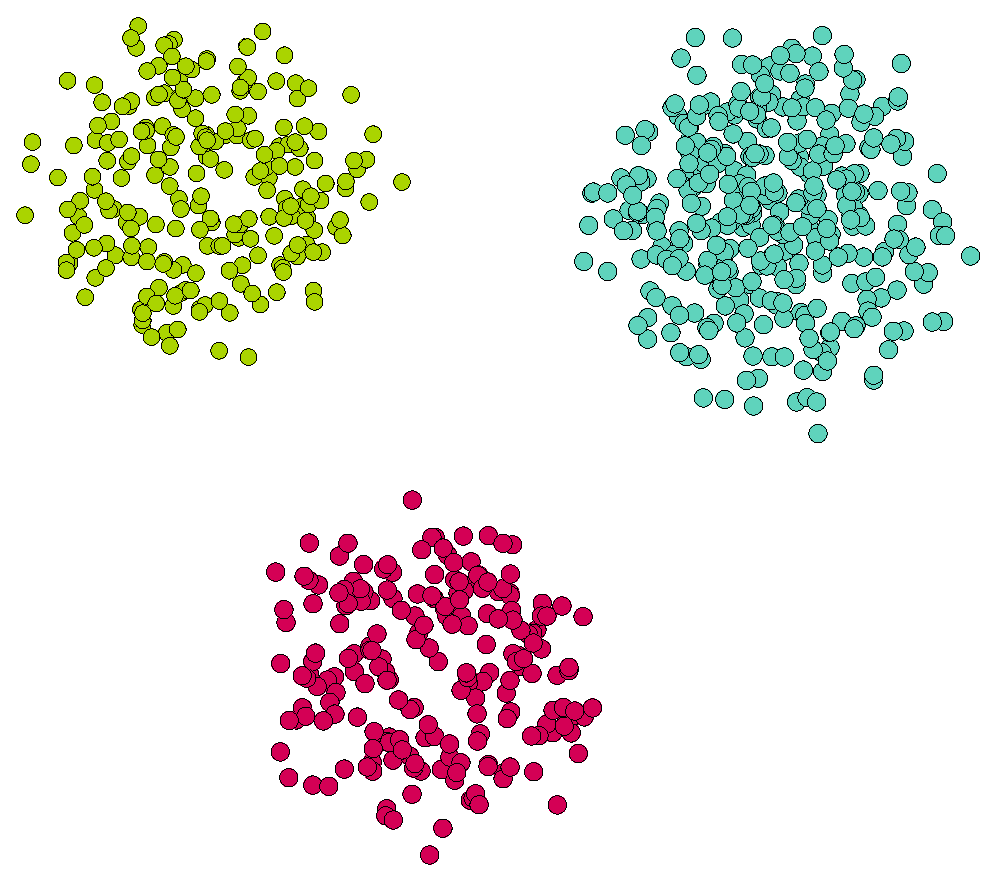
\includegraphics[width=.5\linewidth]{img/wellSeparatedObjects.eps}
  \caption{Well sepatated objects}
  \label{fig:wellSeparatedObjects}
\end{subfigure}
\begin{subfigure}{.49\textwidth}
  \centering
  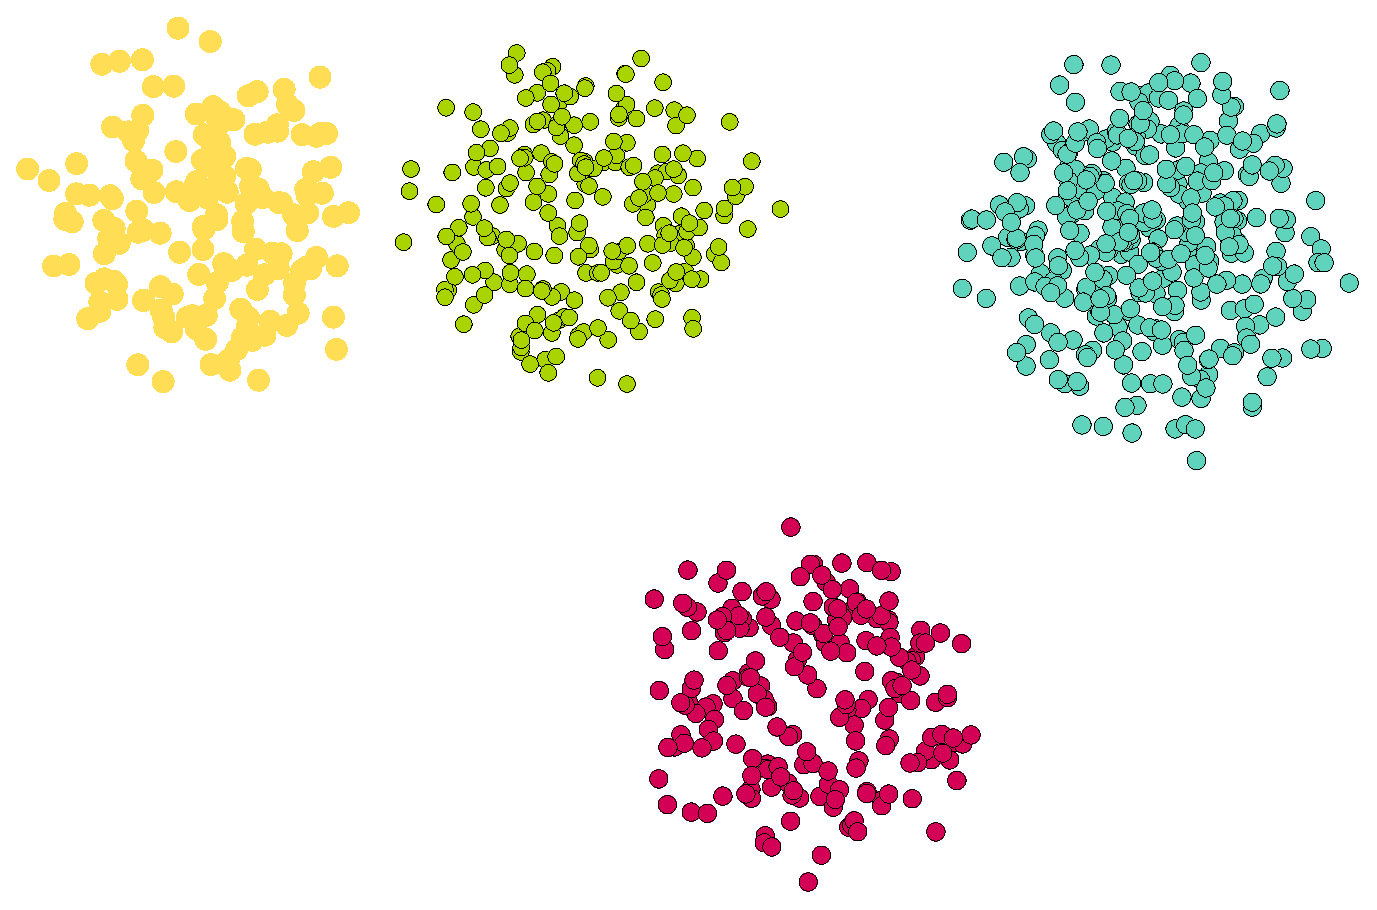
\includegraphics[width=.5\linewidth]{img/centerBasedClusters.eps}
  \caption{Center-Based Clusters}
  \label{fig:centerBasedClusters}
\end{subfigure}
\vspace*{0.5cm} 
\begin{subfigure}{.49\textwidth}
  \centering
  
\includegraphics[width=.5\linewidth]{img/contiguousClusters.eps}
  \caption{Contiguous Clusters}
  \label{fig:contiguousClusters}
\end{subfigure}
\begin{subfigure}{.49\textwidth}
  \centering
  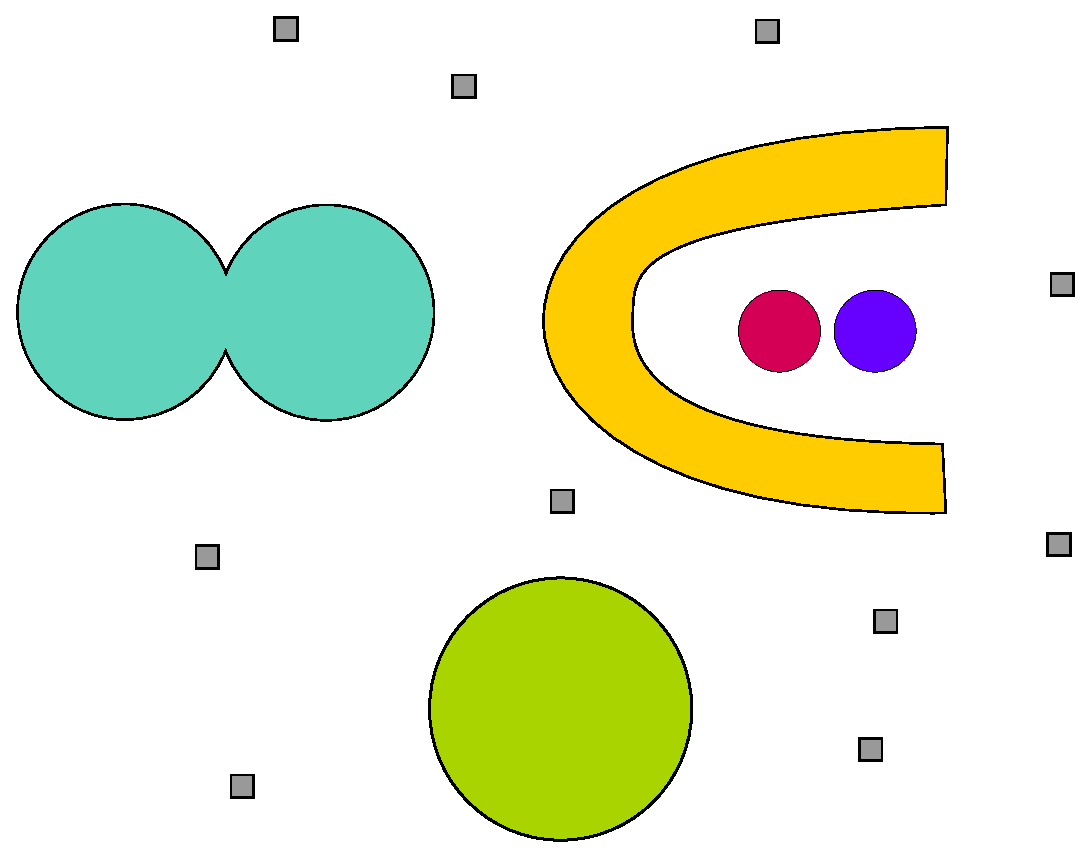
\includegraphics[width=.5\linewidth]{img/densityClusters.eps}
  \caption{Density-Based Clusters (Gray squares represent noise)}
  \label{fig:densityClusters}
\end{subfigure}
\vspace*{0.5cm} 
\begin{subfigure}{.49\textwidth}
  \centering
  
\includegraphics[width=.5\linewidth]{img/conceptualClusters.eps}
  \caption{Conceptual Clusters (Points in cluster have y-coordinate from specific range, omitting x-coordinate)}
  \label{fig:conceptualClusters}
\end{subfigure}
\begin{subfigure}{.49\textwidth}
  \centering
  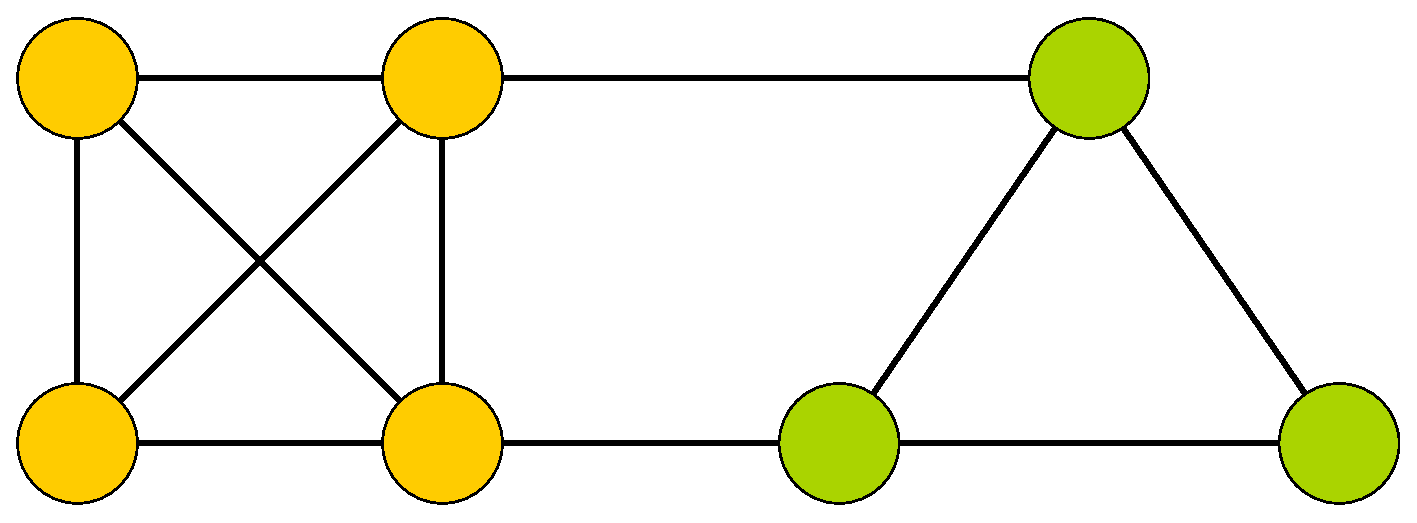
\includegraphics[width=.5\linewidth]{img/graphClusters.eps}
  \caption{Graph-Based Clusters}
  \label{fig:graphClusters}
\end{subfigure}
\caption{Typical cluster models}
\end{figure}

\begin{description}
\item[Well-Separated Clusters] Objects are easily separable-chunks of objects are not overlapping and split by sparse or empty area. Cluster is a set of objects such that each object in cluster is closer to objects from its cluster than to objects from other clusters~\autoref{fig:wellSeparatedObjects}. This is the easiest data input and most of algorithms performs well in this case.

\item[Centroid-Based Clusters] Object belongs to cluster if it is closer to the centroids of the cluster than centroids of all other clusters~\autoref{fig:centerBasedClusters}. Centroid is special object known before or precomputed. The result is similar to Voronoi space partitioning. Centroid-Based clusters are similar Voronoi cells from Voronoi diagram, where centroids are called seed or generators. This is good model for algorithms based on distance between object and centroid. \\
One of the algorithm for solving this task is \textit{\textbf{Centroid-based clustering}} representing clusters as central object, which may not be part of the input data set. This clustering is basically an optimization problem where we looking for centroids so distances will be the lowest possible. Problem is that optimization itself is NP-hard problem and the result only approximate the ideal solution. Approximation is commonly done by many iterations consist of assigning clusters to objects and counting new means.

\item[Contiguous Clusters] This model is similar to Center-Based Clusters model but there is difference that two clusters could be merged into single one if they are close enough~\autoref{fig:contiguousClusters}. In other words, object is in cluster if it is similar to one ore more other objects from cluster~\cite{Tan05}.\\
Main idea of \textbf{Contiguity-based clustering} is that objects that are nearby are more related than objects that are farther, so these algorithms grouping objects based on their distance only. Each cluster can be described by sum of distances or by maximum distance needed to connect objects in cluster. Having these cluster property, they can be easily ordered into hierarchy so parent clusters needs little more distance to connect its objects. This hierarchy could be represented as a dendrogram, which is tree diagram showing cluster hierarchy. Because this property, Contiguity-based clustering could be used for hierarchical clustering but also for hard clustering if we omit the hierarchy.\\

The connection of the objects inside cluster could be problematic. Simply, because cluster consists of many objects, there are many choices to compute the distance to. There are several methods for choosing linkage criteria between two sets of objects $A$ and $B$, $d$ is chosen metric:
\begin{description}
\item[Maximum or complete linkage clustering] $$\max\{d(a,b) : a \in A, b \in B\}$$
\item[Minimum or single linkage clustering] $$\min\{d(a,b) : a \in A, b \in B\}$$
\item[Mean or average linkage clustering, or UPGMA] (Unweighted Pair Group Method with Arithmetic Mean) $$\frac{1}{|A||B|}\sum_{a \in A} \sum_{b \in B} d(a,b)$$
\item[Centroid linkage clustering, or UPGMC] (Unweighted Pair-Group Method using Centroids) $$\|c_a - c_b\| \mbox{ where } c_a \mbox{ and } c_b \mbox{ are the centroids of clusters } A \mbox{ and } B$$
This may look like centroid based clustering but this is only a linkage criteria and the result is hierarchically ordered clusters.
\item[Minimum energy clustering] $$\frac{2}{|A||B|}\sum_{i,j=1}^{|A|,|B|}\|a_i-b_j\|_2-\frac{1}{n^2}\sum_{i,j=1}^{|A|}\|a_i-a_j\|_2-\frac{1}{|B|^2}\sum_{i,j=1}^{m}\|b_{i}-b_{j}\|_{2} : a \in A, b \in B$$
\end{description}

These methods are not resistive for extreme objects, which cause generating new clusters or even merging others. Methods has generally $O(n^3)$ complexity so they are slow for large amount of data. There exist optimization for special cases which has only complexity $O(n^2)$. These methods are taken as obsolete.

\item[Density-Based Clusters] Clusters are dense regions of objects. They are separated by low-density regions. This method is useful when some noise is present because the low-density regions will cover them and clusters will not change.~\autoref{fig:densityClusters} \\
Clusters in \textbf{Density-based clustering} are defined as areas with higher density of objects than in the rest of input data. Standalone objects are taken as noise. One of the most popular method is \textit{DBSCAN}. It is similar to contiguity-based clustering, because it connecting points based on the distance, but it only connects points satisfying density criterion. This means that in neighborhood specified by distance must be a minimum number of objects. These objects are called core objects and form the basis of cluster. Than objects which do not satisfy the density criterion but are close enough to at least one point from the cluster are added to cluster too.\\
The advantage of this method is its computational unpretentiousness, because it require only linear number of range queries. This method is deterministic so there is no need to run it in iterations.
Drawback of these methods is the $\epsilon$ density parameter so borders of clusters with smaller density could be interpreted as  noise. Also separating nearby clusters may cause problems to these methods.

\item[Distribution models] Clusters in distribution models are objects that belong to same probability distribution. It is possible that one object belongs to more clusters.\\
In \textbf{Distribution-based clustering}, clusters are defined as objects from the same or similar distribution. This approach basically emulates process of generating the input data and try to reconstruct the lost statistical parameters. Main problem of this clustering model is problem known as \textit{overfitting}. This means that more complex model is described by less complex one and the difference between them is marked as deviation or noise. For example 3 points from the neighborhood of parabola vertex will be described by linear function.\\
One of methods used in distribution-based clustering is \textit{Gaussian mixture models} where algorithm iteratively optimizing parameters of fixed number of Gaussian distributions.
Problem is that this method assuming Gaussian distributed data set, but this set may not have even a model.

\item[Conceptual Clusters] Objects in cluster has some properties same or similar, but other properties could differ significantly.~\autoref{fig:conceptualClusters}\\
As algorithm for Conceptual Clusters, we can use algorithm depends on other model properties and less significant properties of objects could be easily filtered out.

\item[Graph-Based Models] For example cliques in graphs should represent clusters. Clique is subset of nodes where every two nodes are connected with edge.~\autoref{fig:graphClusters}\\
Because of special demands of this model, special algorithms are needed so we could use graph algorithms, for example Bron-Kerbosch~\cite{Sun15} algorithm for finding cliques.
\end{description}

\subsection{K-Means} 
Clustering algorithms are wide class of algorithms and we could not focused on every clustering model and appropriate algorithm and speed it up by parallelization, because there does not exist any universal approach for speeding up but on the contrary it needs to use every single detail of the algorithm. We want to choose one of the most versatile algorithm so we decided for k-means algorithm for its wide range of usage and undemanding on the properties of the input data.\\
K-means algorithm~\cite{Aggarwal13,Tan05} is centroid based clustering algorithm. K-means input is set of $n$ points in $d$-dimensional space $R^d$, a number of output clusters $k$ and a optional number of maximum iterations $i$. \\
The task is to assign points to centroids (centers of clusters) and minimize the distance between cluster's centroid and points assigned to this cluster. Algorithm works iteratively and each iteration consist of two steps. At first step the nearest centroid is found for each point and this point is assigned to centroid's cluster. In the second step, new centroids are computed as a mean of all points assigned to same cluster. Algorithm ends after known number of steps or when nothing changes between two iterations.\\
Output of the this algorithm are centroids coordinates and points with assigned clusters.


\algdef{SE}[REPEAT]{Repat}{Until}{\algorithmicrepeat}[1]{\algorithmicuntil\ #1}

\begin{algorithm}
\caption{K-means}\label{alg:kmeans}
\begin{algorithmic}[1]
\State Select K points as the initial centroids
\Repeat
\State Make K clusters by assigning all points to the nearest cluster
\State Update centroid of each cluster
\Until{centroids do not change or maximum number of iterations reached}
\end{algorithmic}
\end{algorithm}

Because at first step we do not know the centroids, usually, the first $k$ points of input set are used as initial centroids. K-means converge fast in first few iterations, so the stopping condition could be changed to ``Until relatively few points change clusters''.~\cite{Tan05}.\\
The complexity of the computation is $O(n*k*i*d)$, where $n$ is number of input points, $k$ is number of clusters, $i$ is number of iterations and $d$ is dimension of space.\\

To evaluate k-means output, we need to somehow measure the quality of cluster assignment. For this purpose is most commonly used \textbf{Sum of Squared Error (SSE)} function. Single point error is represented by distance from the centroid of assigned cluster and the function than sums square errors of all points.
$$SSE = \sum^k_{i=1}\sum_{o \in O_i}|o,c_i|^2, \textrm{ $c_i$ \textit{is centroid of cluster} $O_i$ }$$
If we had results with bad $SSE$, we could reduce it by increasing number of clusters $k$, but this may not help if initial clusters are chosen badly.

The initial centroids are one of the disadvantages of k-means algorithm because we need to know the number of output clusters at the beginning and after computation start this number could not be changed. This possibility might be demanded by some type of problems and k-means is inconvenient for them. In addition to that, problem is also selecting of initial centroids. Although we choose ideal $k$ for the input data, the probability we chose objects from different clusters as initial points is really small~\cite{Tan05}: $$P = \frac{\mbox{number of ways to select one centroid from each cluster}}{\mbox{number of ways to select K centroids}}=\frac{k!{n \choose k}}{k^k {n \choose k} }=\frac{k!}{k^k}$$ This probability is close to zero even for small $k$, for example for $k=10$, probability is $0.00036$.\\
There are some ways to solve this problem and pickup better initial points~\cite{Tan05}:
\begin{description}
\item[multiple runs] k-means algorithm is run multiple times with different initial centroid and the best one is chosen.
\item[samples] Sample input data with hierarchical clustering and determine initial centroids.
\item[more centroids] Select more than $k$ centroids and then selects the most widely separated ones.
\item[postprocessing] Result of the algorithm is postprocessed - Clusters with high $SSE$ could be split and on the other side close clusters with low $SSE$ could be merged.
\end{description} 

Other problem of k-means is that the basic version could produce empty clusters. This could be solved by algorithm update: when we found empty cluster, we could choose point which contributes most to $SSE$ as centroid instead of empty cluster or we can choose point from the cluster with greatest $SSE$~\cite{Tan05}.

Also if clusters differs significantly in size/density/non-globular shapes~\cite{Tan05}, cluster analysis could be problem for k-means\\
For example, because the main goal of k-means is to produce similar sized clusters, we will have problem with input data where one big cluster contains many objects and one smaller cluster has only few objects~\autoref{fig:kmeansbadinputsize}. Than k-means divide the bigger cluster~\autoref{fig:kmeansbadoutputsize} so some objects from bigger that are closer centroid to smaller cluster are assigned to smaller cluster which could be undesirable because k-means ignores input data distribution.
\begin{figure}[h]
\centering
\begin{subfigure}{.49\textwidth}
  \centering
  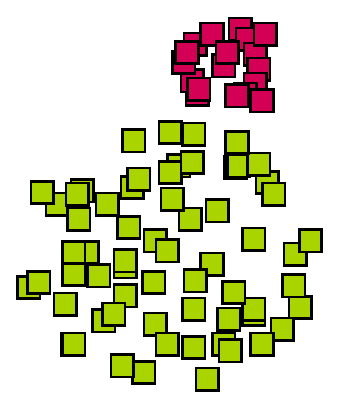
\includegraphics[width=.5\linewidth]{img/kmeans_badInputSampleSize.eps}
  \caption{Input data (assigned to clusters only for demonstration)}
  \label{fig:kmeansbadinputsize}
\end{subfigure}
\begin{subfigure}{.49\textwidth}
  \centering
  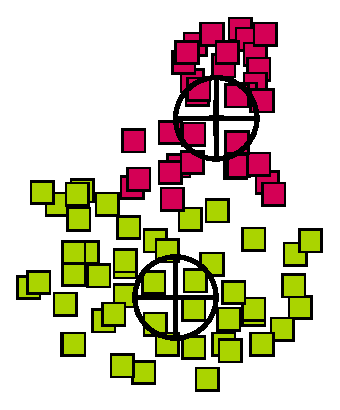
\includegraphics[width=.5\linewidth]{img/kmeans_badOutputSampleSize.eps}
  \caption{k-means output}
  \label{fig:kmeansbadoutputsize}
\end{subfigure}
\caption{K-means bad sized samples}
\end{figure}

Next problem is caused by cluster density. When we have some close dense clusters and cluster signle sparse cluster~\autoref{fig:kmeansbadinputdensity}, k-means usually mark dense clusters as one and split sparse cluster into multiple clusters.~\autoref{fig:kmeansbadoutputdensity}
\begin{figure}[h]
\begin{subfigure}{.49\textwidth}
  \centering
  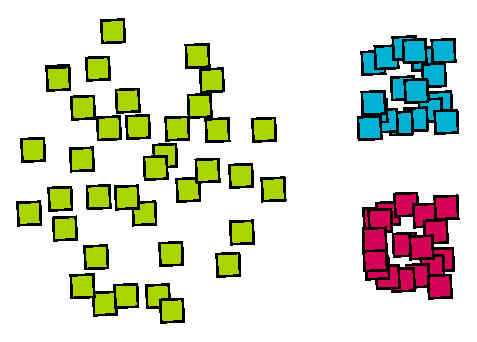
\includegraphics[width=.5\linewidth]{img/kmeans_badInputSampleDensity.eps}
  \caption{Input data (assigned to clusters only for demonstration)}
  \label{fig:kmeansbadinputdensity}
\end{subfigure}
\begin{subfigure}{.49\textwidth}
  \centering
  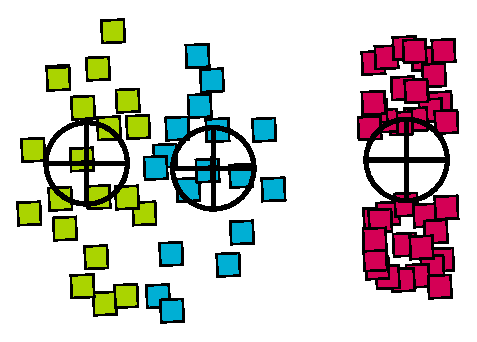
\includegraphics[width=.5\linewidth]{img/kmeans_badOutputSampleDensity.eps}
  \caption{k-means output}
  \label{fig:kmeansbadoutputdensity}
\end{subfigure}
\caption{K-means bad density clusters}
\end{figure}

Other problem is that k-means algorithm does not recognize cluster shape and produce only globular clusters. This could be problem when two usually non-convex clusters~\autoref{fig:kmeansbadinputshape} are close enough and one interferes into convex hull of the other. Than, k-means usually assigns points from one cluster to another and vice versa~\autoref{fig:kmeansbadoutputshape}.
\begin{figure}[h]
\begin{subfigure}{.49\textwidth}
  \centering
  
\includegraphics[width=.5\linewidth]{img/kmeans_badInputSampleShape.eps}
  \caption{Input data (assigned to clusters only for demonstration)}
  \label{fig:kmeansbadinputshape}
\end{subfigure}
\begin{subfigure}{.49\textwidth}
  \centering
  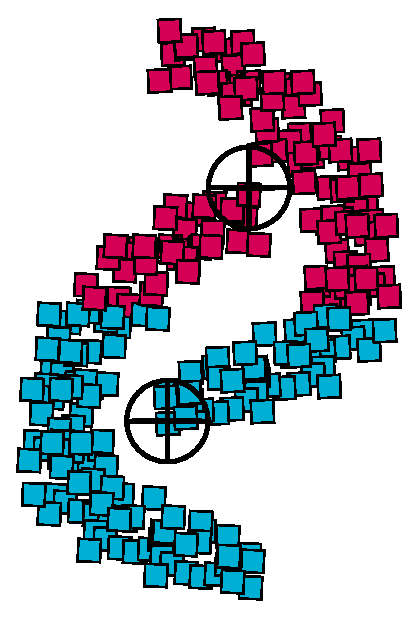
\includegraphics[width=.5\linewidth]{img/kmeans_badOutputSampleShape.eps}
  \caption{k-means output}
  \label{fig:kmeansbadoutputshape}
\end{subfigure}
\caption{K-means non-globular clusters}
\end{figure}

These problems could be solved by using more clusters than input data naturally requires. For example, input data~\autoref{fig:kmeansbadinputshape} contains two natural clusters, but when we try to split data into more clusters, the result will contain small clusters which contain only points from single original cluster and not from the other one~\autoref{fig:kmeansbadoutputsolution}. If we post process this data, we could get expected result and prevent this k-means deficiency.
\begin{figure}[h]
  \centering
  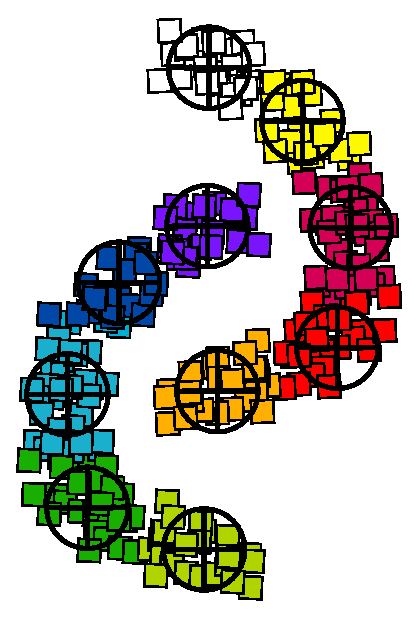
\includegraphics[width=.3\textwidth]{img/kmeans_badOutputSampleShapeSolution.eps}
  \caption{K-means solution for bad shaped cluster}
  \label{fig:kmeansbadoutputsolution}
\end{figure}


\subsubsection{K-Means Variants}
Because k-means is universal algorithm, there exists some variants if classical k-means algorithm is inconvenient or unusable. These variants could solve some problems and limitations of classical k-means algorithm.
\begin{description}
\item[k-medoids] - centroids are not virtual points in $R^d$ space but point from input data whose average dissimilarity to all other objects in cluster is minimal (medoid is used instead of mean).
\item[k-medians] - same algorithm as k-means, but in each dimension, median is used instead of mean for computing new centroid.
\item[k-means++] - initial centers are chosen randomly. This selection avoid bad inputs.
\item[Fuzzy C-means] - fuzzy cluster~\ref{sec:clusterorganization} assignment is allowed. Object does not belong strictly to one centroid but it has degree of belonging to cluster. The weighted mean (with the degree of belonging as weight) is used for computation new centroids.
\item[Bisecting k-means]~\cite{Tan05} is variant of k-means, which produce hierarchical clustering.It works also iteratively as k-means, but in each step, the clusters with highest SSE is bisected by classical k-means algorithm with $k=2$. The algorithm iterates until it reaches the number of needed clusters.~\autoref{alg:bisectingkmeans}
\begin{algorithm}
\caption{Bisecting k-means}\label{alg:bisectingkmeans}
\begin{algorithmic}[1]
\State Insert all points into the list of clusters as single cluster
\Repeat
\State Select first cluster from the list of clusters
\For{i=1 to number of iterations}
\State Bisect selected cluster using k-means algorithm
\EndFor
\State Add the two clusters from the bisection with the lowest SSE to the list of the clusters
\State Update centroid of each cluster
\Until{list of clusters contains k clusters}
\end{algorithmic}
\end{algorithm}

\end{description}

%\chapter{General-Purpose Computing on Graphics Processing Units}
General-Purpose computing on graphics processing unit (GPGPU) is the utilization of graphics processing unit (GPU), which was originally designed for computer graphical computations, to cooperate with central processing unit (CPU) on general tasks which are normally processed only by CPU.\\
Because solving graphical tasks require many vector or matrix computations, which are naturally parallel, GPU's architecture contains many simple cores capable of basic mathematical operations and parallel work. This is their main advantage in comparison with ordinary CPU - they have ten times, a hundred times but lately thousand times more cores designed to work in parallel, so if the task is well parallelizable, it could be accelerated up to hundred times on GPU in comparison to serial CPU version.\\
At the beginning of GPGPU, cards support only computation of vectors or matrices, usually two, three or four dimensional because these structures are commonly used in graphics computations, so general purpose computation had to be reformulated to this graphical principles supported by major graphics APIs like DirectX or OpenGL. This transformation was hard for programmer and very often impossible, so many algorithms could not be transfered to graphical problems and could not be parallelized on GPUs.\\
This problem disappears later with the arrival of specialized frameworks for utilizing GPUs for general purpose programming. These frameworks allows to programmer hides limitations of graphics environment and make general computations easier.~\cite{Kirk12}\\
Nowadays there exist two major frameworks for GPGPU - CUDA~\cite{Sanders10} and OpenCL~\cite{Scarpino11} (open computing language). The main advantage of CUDA is a direct link to the hardware, which is not the case of OpenCL and others. This is because CUDA is developed by Nvidia and only for Nvidia graphics cards so it could use concrete hardware specific properties. Compared to that, OpenCL by Khronos group is a universal, vendor independent framework for parallel computations supporting a large range of hardware divergent devices - it can be run on many CPUs and GPUs including Nvidia. This wide support of devices is a problem for high performance computing because OpenCL could not use every property of concrete architecture and hardware simply because there is nothing like concrete architecture. In the opposite CUDA is designed only for cards by Nvidia so it benefits from a small range of supported devices. In this work, we decided to use CUDA for one of the best performances among other frameworks and because we will not take main OpenCL advantage, the portability.\\
Other advantage of CUDA is that the device code and host code are written together and that they are both compiled in compile time in difference to OpenCL which compile device code at runtime.

\section{GPU architecture}
GPU is multi-processor highly tuned for graphics which demands fast processing of many floating point operations. Physically, it could be placed on special graphical card connected to mother board usually by PCI Express bus or it could be placed directly on CPU chip. Because GPUs integrated into CPU are not so powerful, we will focus on external graphical cards. Directly on graphical card are GPU chip and also memory to reduce memory latency. GPU usually consists of following components:
\begin{description}
\item[unified shaders] are programmable execution units responsible for computations. They replaced specialized shaders like vertex shaders or pixel shaders. Due to unification, the workload could be better balanced and for example tasks with many geometry computations, system can allocate most computing units for geometry shaders. Because of unification, also non-graphical tasks could be computed on GPUs.
\item[memory controller] is responsible for communication between GPU and graphical memory.
\item[texture mapping unit] is placing textures on objects
\item[render output unit] makes the final image sent to output device.
\end{description}
For GPGPU computations, only unified shaders and memory (memory controller) is used.

\subsection{GPU and CPU comparison} \label{ssec:gpucpucomparison}
Main difference between CPU and GPU is in their specialization. Instead of general purpose of CPUs, GPUs are specialized on graphics. Graphical computations requires high throughput of data, so their architecture is targeted for massive parallel calculations with numbers. The single cores are significantly different too because CPU core usually works on higher frequency (about 2 - 3 GHz) and supports many instructions in comparison to GPU core which works on lower frequencies (800 - 1000 MHz) and supports only special set of instructions. Problem was the special designation of GPUs but after GPGPU was introduced, problem with GPU specialization was solved by special frameworks and GPUs began to compete with processors. Main differences between CPUs and GPUs are:
\begin{description}
\item[Number of cores] CPU has only few physical cores~\autoref{fig:cpuarchitecture}. Common CPUs have up to 8 logical cores, server CPUs could have more, but usually it is between 8 and 12 cores on chip. Compared two that, modern GPUs have around thousand CUDA cores~\autoref{fig:gpuarchitecture}, the top models have thousands of cores (for example, GeForce GTX Titan X has CUDA cores), so they have great potential for parallel tasks.
\item[Core architecture] GPU cores are specialized for numeric computations, not for general tasks as CPU cores. This is not so big limitation of GPU, because the are usually used for numeric computations. CPU advantage is frequency, usually, CPU core is five times faster than GPU core. But because of specialized optimizations, which allows certain calculations to go much faster than on CPU, lower frequency is not a problem. The lesser frequency of GPU has several reasons, for example it is really hard to take away heat generated by thousands of cores placed on single chip and  because higher frequencies generates more heat, GPU can not run on faster frequencies like CPU.
\item[Threads] Approach to threads is also different. CPU can process different instructions at one time, which is called Simultaneous Multithreading (SMT), GPU multiprocessor is capable of running multiple threads, but with same code, because execution units shares single fetch/decode unit.
\item[Memory] CPUs use big cache memory for hide latency of memory access so when thread is switched to different core, there is problem with locally cached data, which could be useless (depend on cache type) on original core and must be re-cached on new core. GPU has only smaller caches, but the threads are not switched between cores.
\end{description}

\begin{figure}[h]
\centering
\begin{subfigure}{.49\textwidth}
  \centering
  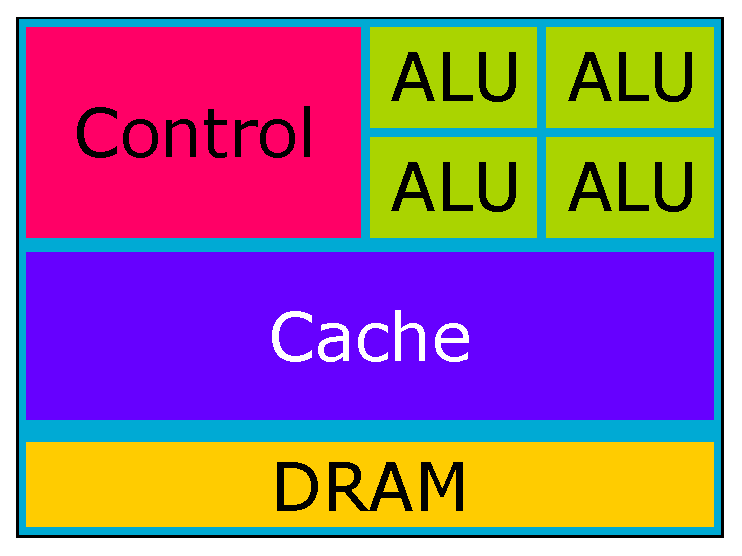
\includegraphics[width=1\linewidth]{img/CPUarchitecture.eps}
  \caption{CPU architecture}
  \label{fig:cpuarchitecture}
\end{subfigure}
\begin{subfigure}{.49\textwidth}
  \centering
  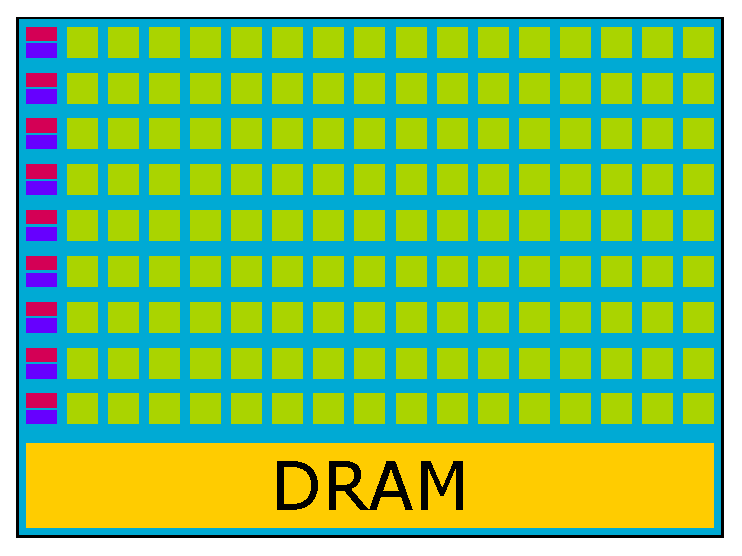
\includegraphics[width=1\linewidth]{img/GPUarchitecture.eps}
  \caption{GPU architecture}
  \label{fig:gpuarchitecture}
\end{subfigure}
\caption{CPU and GPU architecture comparison (same colors of boxes in GPU means same units)}
\end{figure}

%\begin{table}
%\begin{tabular}{|l|l|l|}
%\cline{1-2}
%NIC & CPU & GPU \\ \cline{1-2}
%# cores & Few cores per chip & Many cores per chip \\ \cline{1-2}
%Specialization & General purpose cores & Cores psecialized for numeric computations \\ \cline{1-2}
%Threads approach & Processing different threads & SIMT thread processing \\ \cline{1-2}
%Memory access & Huge caches to reduce memory latency & Huge amount of threads and fast context switch \\ \cline{1-2}
%\end{tabular}
%\end{table}
\section[Compute Unified Device Architecture]{Compute Unified Device Architecture\\ (CUDA)}
CUDA is parallel computing platform for GPGPU developed by Nvidia including hardware and software architecture integrated on Nvidia graphics cards. CUDA programs could be written in C, C++ and Fortran programming languages which make it easy for programmer. There exist more solutions than this one from Nvidia, but CUDA is one of the most used for its high performance computing.For example programs in OpenCL, CUDA competitor, is translated to CUDA functions on Nvidia graphics cards.\\

\begin{figure}[h]
\centering
%\begin{subfigure}{0.49\textwidth}
%  \centering
%  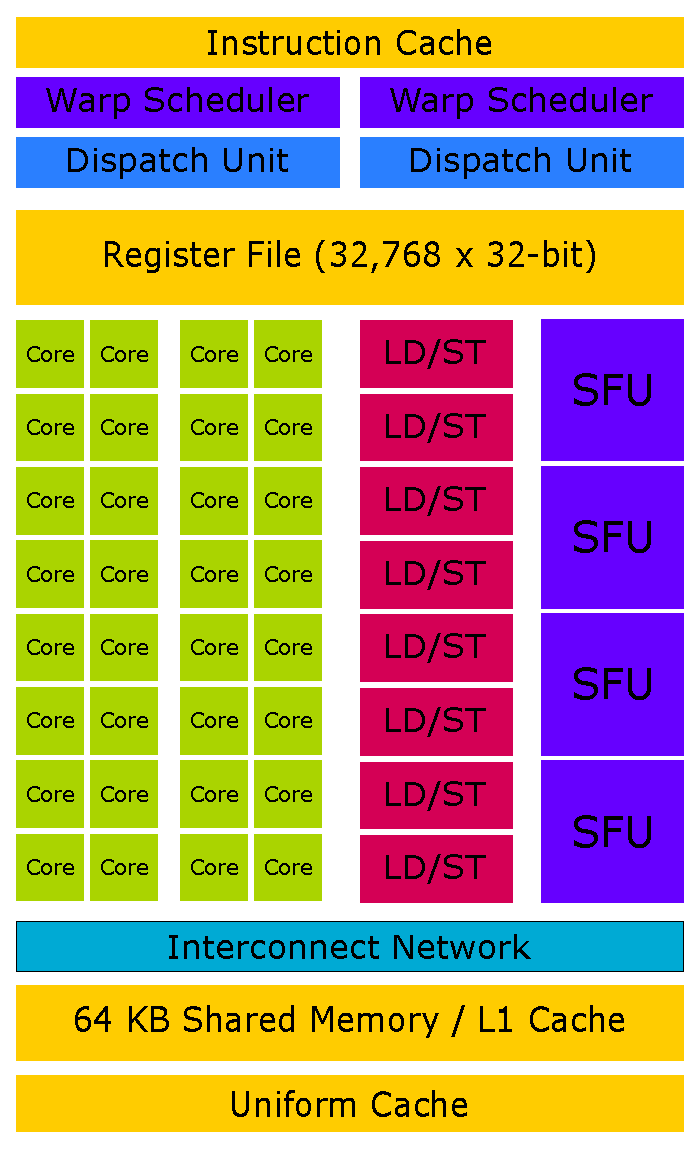
\includegraphics[width=0.8\linewidth]{img/SMPArchitecture.eps}
%  \caption{SMP architecture (Fermi)}
%  \label{fig:smparchitecture}
%\end{subfigure}
%\begin{subfigure}{0.6\textwidth}
  %\centering
  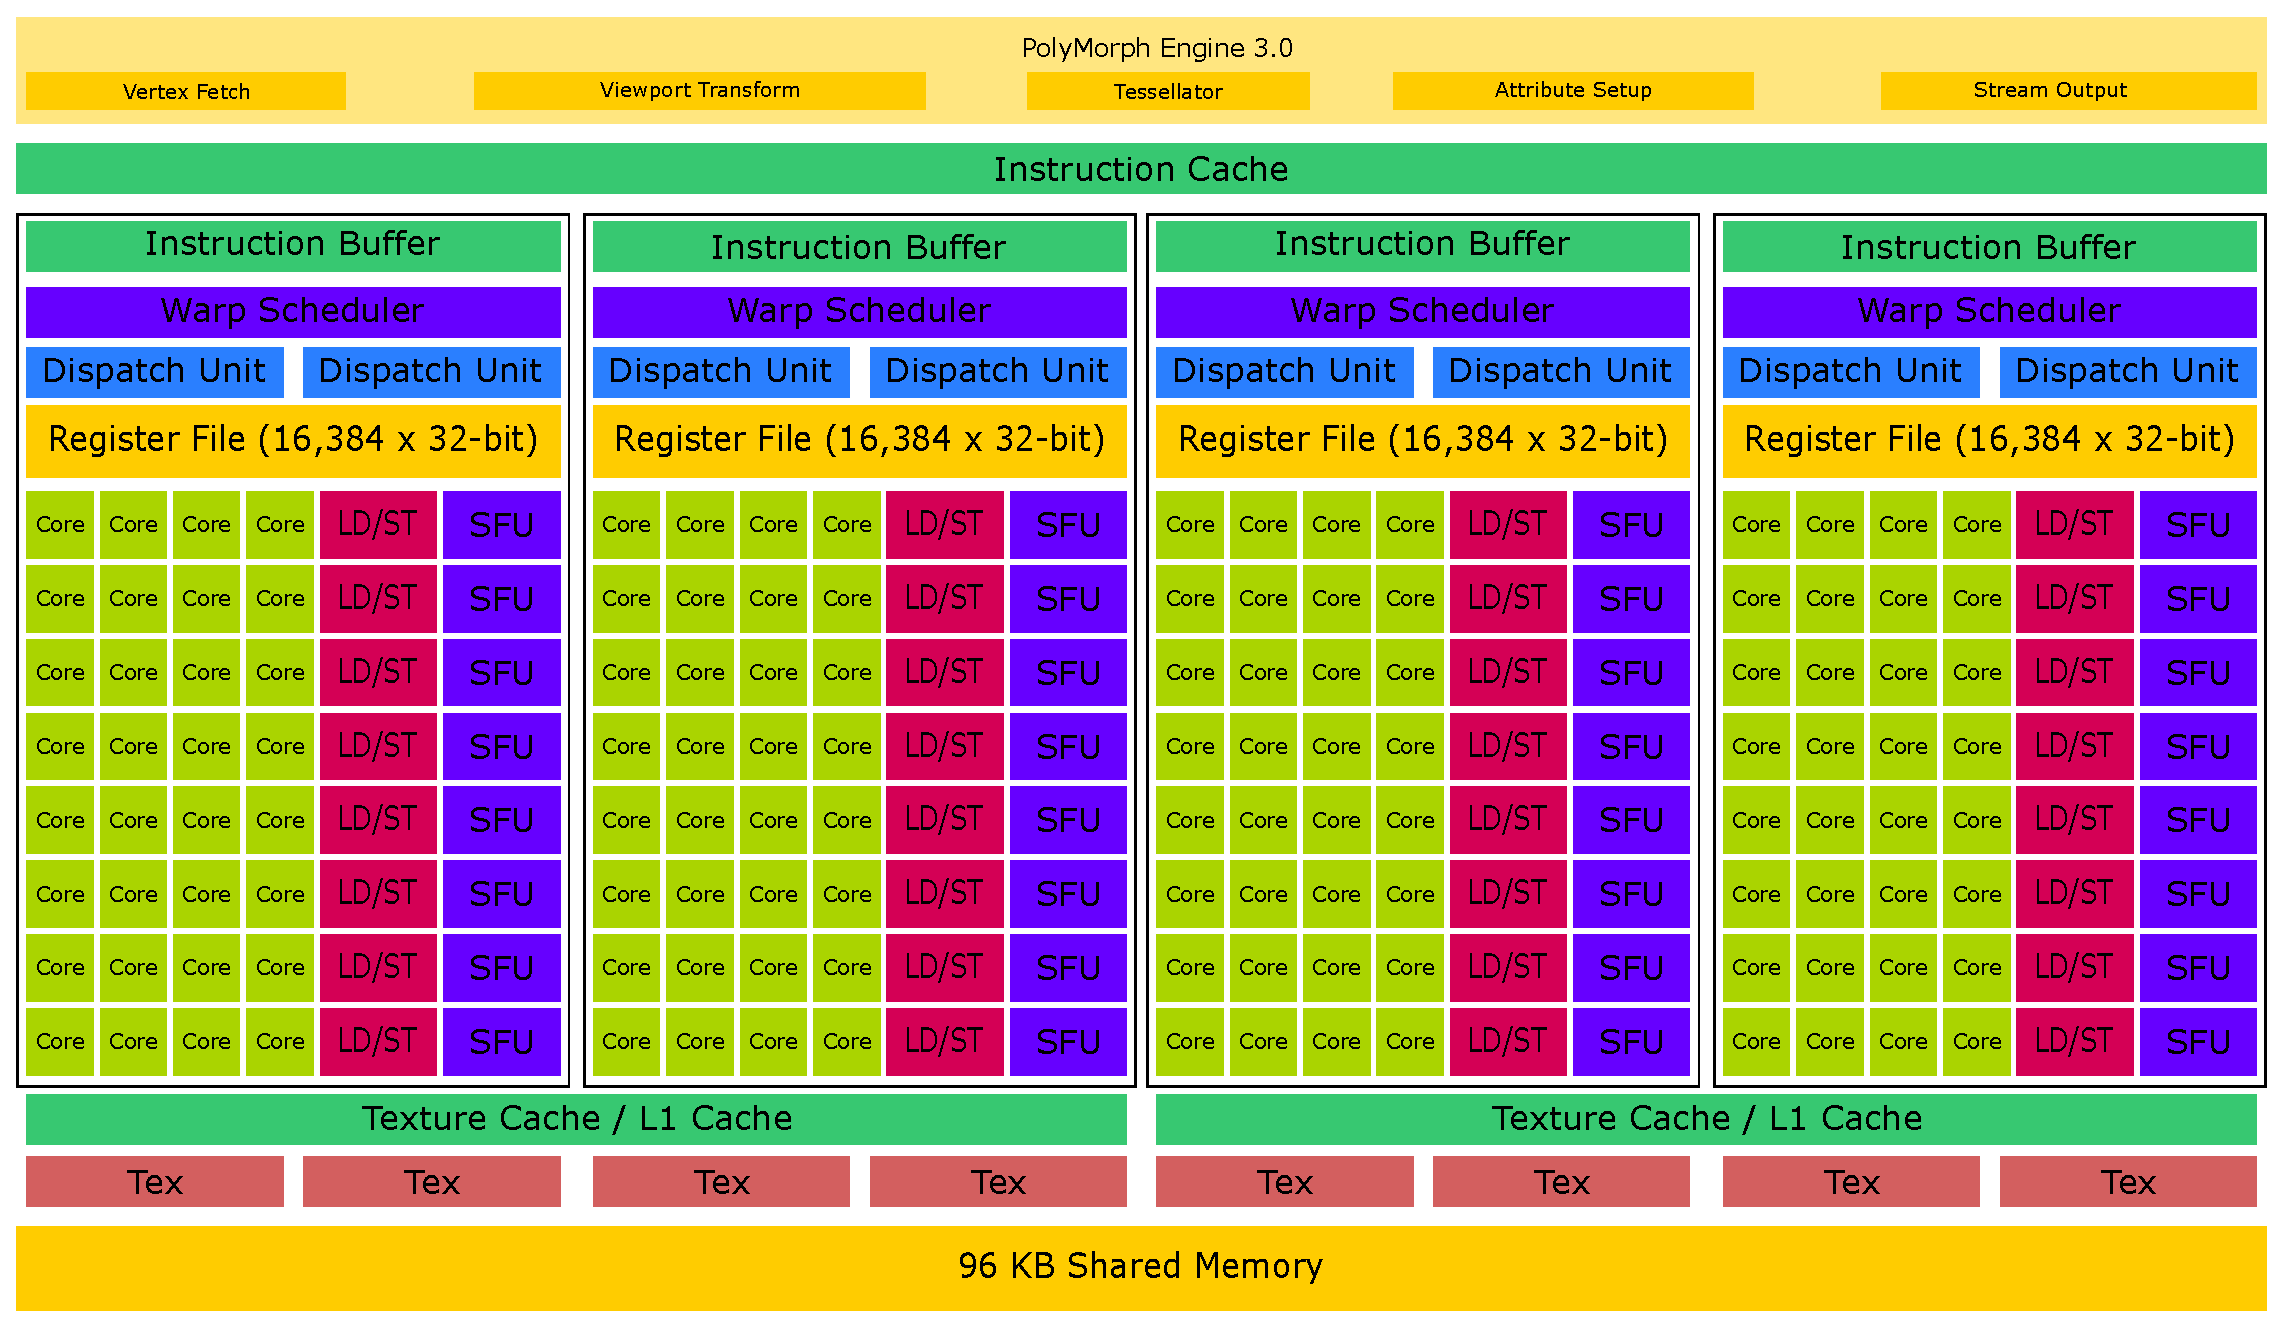
\includegraphics[width=1\linewidth]{img/SMMArchitecture.eps}
  \caption{SMM architecture (Maxwell)}
  \label{fig:smmarchitecture}
%\end{subfigure}
%\vspace*{0.1cm} 
%\begin{subfigure}{0.6\textwidth}
%  \centering
%  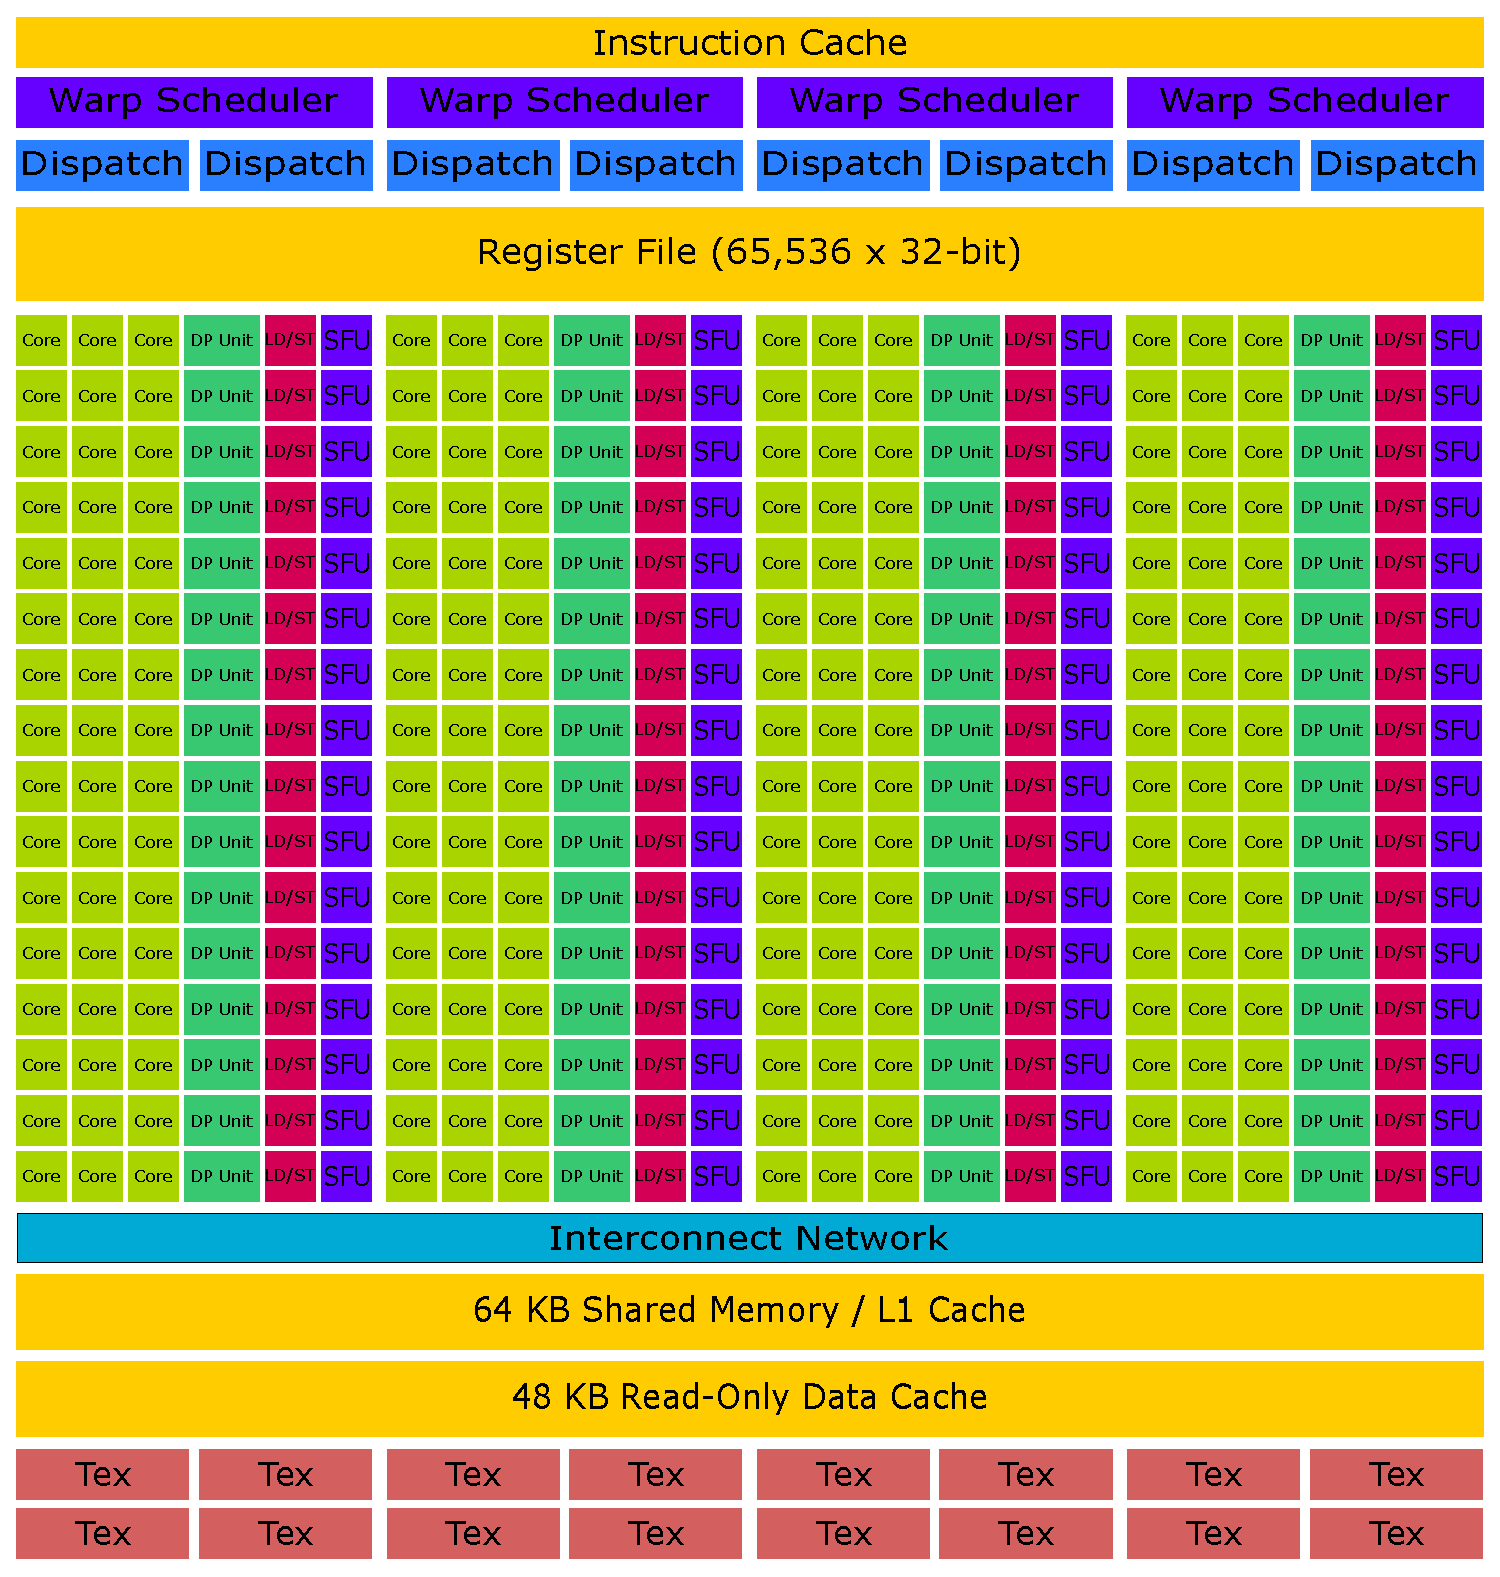
\includegraphics[width=0.9\linewidth]{img/SMXArchitecture.eps}
%  \caption{SMX architecture (Kepler)}
%  \label{fig:smxarchitecture}
%\end{subfigure}
\end{figure}

CUDA architecture contains larger processors called \textbf{Streaming Multiprocessor (SMP)}. The oldest is \textbf{SM} - Fermi, \textbf{SMX} - Kepler and the newest \textbf{SMM} - Maxwell~\autoref{fig:smmarchitecture}. Each SMP contains processor cores with registers (from 32 on Fermi architecture, 128 on Maxwell architecture and 192 on Kepler architecture), load/store units (LD/ST), Special Function Units (SFUs), shared instruction cache, shared memory and data caches. LD/ST and SFUs are shared by groups of cores, size of group depends on architecture.

\begin{figure}[h]
  \centering
  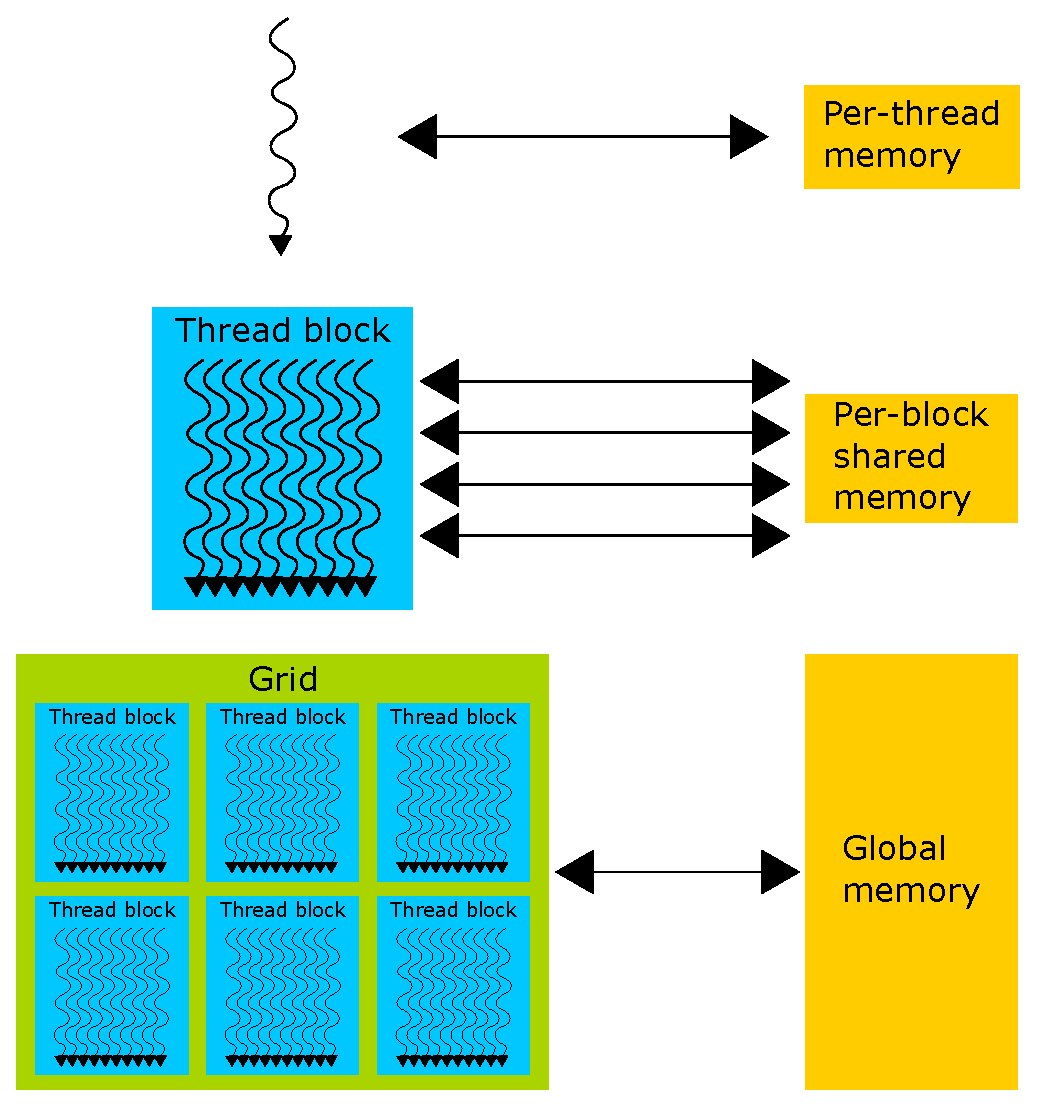
\includegraphics[width=0.8\linewidth]{img/CUDAmemoryHierarchy.eps}
  \caption{CUDA Execution model}
  \label{fig:cudamemhierarchy}
\end{figure}

Next different parameter of CUDA device is \textbf{Compute Capability} (CC), which describes the device characteristics and a set of instructions that are supported. CC is tightly coupled with architecture (CC 1.x was supported by Tesla architecture, CC 2.x by Fermi, 3.x by Kepler, 5.x by Maxwell).\\

CUDA use Simple Instruction Multiple Thread (SIMT) model. This model approaching parallelism by broadcasting same instruction to multiple execution units, so only one instruction fetch/decode unit is needed for group of execution units. This model is similar to Simple Instruction Multiple Data (SIMD) model, but the difference is that SIMT also have multiple register sets. Main difference is that SIMD processes short vectors in parallel and always all threads do the same work. For example, when we need sum two vectors, SIMD must iterate through vectors and in one step, it can only process as many elements as a computing units count is. On CUDA with SIMT model, we launch as many threads as size of vector and each thread can store values in own register.\\

\subsection{CUDA Workflow}
When we want to launch CUDA program, first think what we must do in host code is detect CUDA capable devices. When desired device is selected, we could start with copying data from host to device. This action is asynchronous so we must synchronize execution of host code and memory transfer. When data transfer is done, we could launch device code called \textbf{kernel}. Kernel is same as normal C function but defined with special declaration and it can use special device functions specified by CC. \\
Kernel is launched from host code same as normal function but it runs asynchronously. This function is executed $N$ times in parallel by different CUDA threads. Number of threads is specified at function call. Threads are arranged in one, two or three dimensional space so it could easily reflect data structures like vectors, matrices or volumes. This bunch of threads is called \textbf{block}. The number of threads in block is limited because all threads in block must reside on the same streaming multiprocessor and must share its limited memory resources so on current GPUs, maximum number of threads is 1024.\\
The total number of threads is multiplied by number of blocks. Blocks could be also arranged in one, two or three dimensional space. Only limitation is that each block must be equally shaped so usually the number of thread blocks is determined by size of data being processed or by total number of cores. The total number of threads which are executed in single kernel is number of threads times number of blocks as specified on~\ref{fig:cudagridthreadblock}. Kernel is also called asynchronously so when kernel is executing, host could for example start another memory transfer or doing another work on CPU. After synchronizing with device, we need usually transfer results from the device back to host which is again asynchronous call and must be synchronized.

\begin{figure}[h]
  \centering
  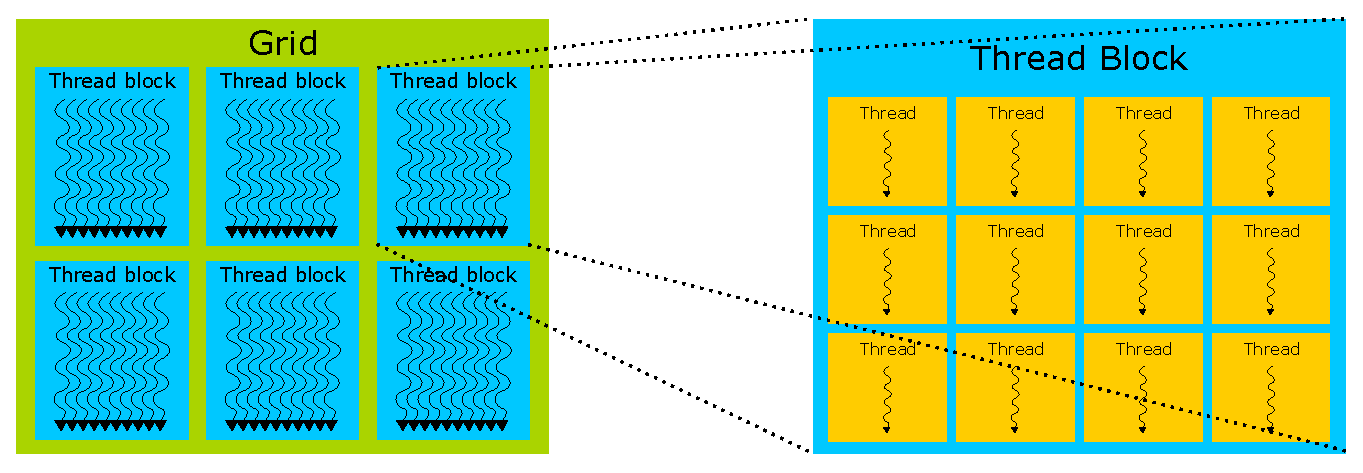
\includegraphics[width=1\linewidth]{img/CUDAthreadGridBlock.eps}
  \caption{2-dimensional grid of 2-dimensional thread blocks}
  \label{fig:cudagridthreadblock}
\end{figure}

Because number of cores is usually smaller than number of threads specified on kernel launch, only some threads could be run in parallel. These groups of threads are called \textbf{Warps}. When Kernel is launched, each block is assigned to SM and does not migrate to another SMP. Than, Each SMP splits its blocks into Warps depends on architecture. Warp threads are executed simultaneously by SMP cores. Splitting of the work between blocks and threads could significantly change the performance, because when we choose bad size of block (indivisible by Warp size) some Warps will not use all cores of single SMP. for example, if we launch same kernel with 8 blocks of 96 threads, block will be split into 3 warps which will be executed in parallel so we will have 24 warps to compute. Compare to that, if we launch the same kernel with 64 blocks of 12 threads, each block will be represented by warp containing only 12 threads so the total number of warps for execution will be 64 because CUDA is not capable to coalesce threads from different blocks. For this reason, it is recommended to set the size of the block to number divisible by size of Warp.\\
There are limitations for operations which could be run in parallel. For example, on Kepler architecture, only 4 of the 12 groups of cores can execute double precision operations at one time, so the slowdown of double precision computation may be up to 3 times. However, the other 8 groups could perform integer or float operations so the slowdown is usually smaller.\\
Problematic are problems with memory operations. Common CPU hides these latency by multilevel cache memory. CUDA architecture also contains some memory caches~\ref{fig:cudamemhierarchy} but because of the most common specialization of algorithms accelerated on GPU - stream or throughput computing, memory caching is ineffective. On CUDA, this is problem is reduced by more active warps on one core so when one warp stalls on memory operation, SMP switches to another ready warp. This mechanism keeps computing cores busy as possible and increasing the efficiency of computation.\\
Threads in single block are executed on a single SM. They share caches and could be synchronized across the threads from same warp. Compared to that threads from different Thread Blocks could be assigned to different SMPs or on same SMP concurrently. They could be even assigned to different or same SM at different times.

\subsection{Memory model}

Memory model on CUDA architecture~\ref{fig:cudamemaccess} contains more types of memory which differs mainly in size, bandwidth and latency.

\begin{figure}[h]
  \centering
  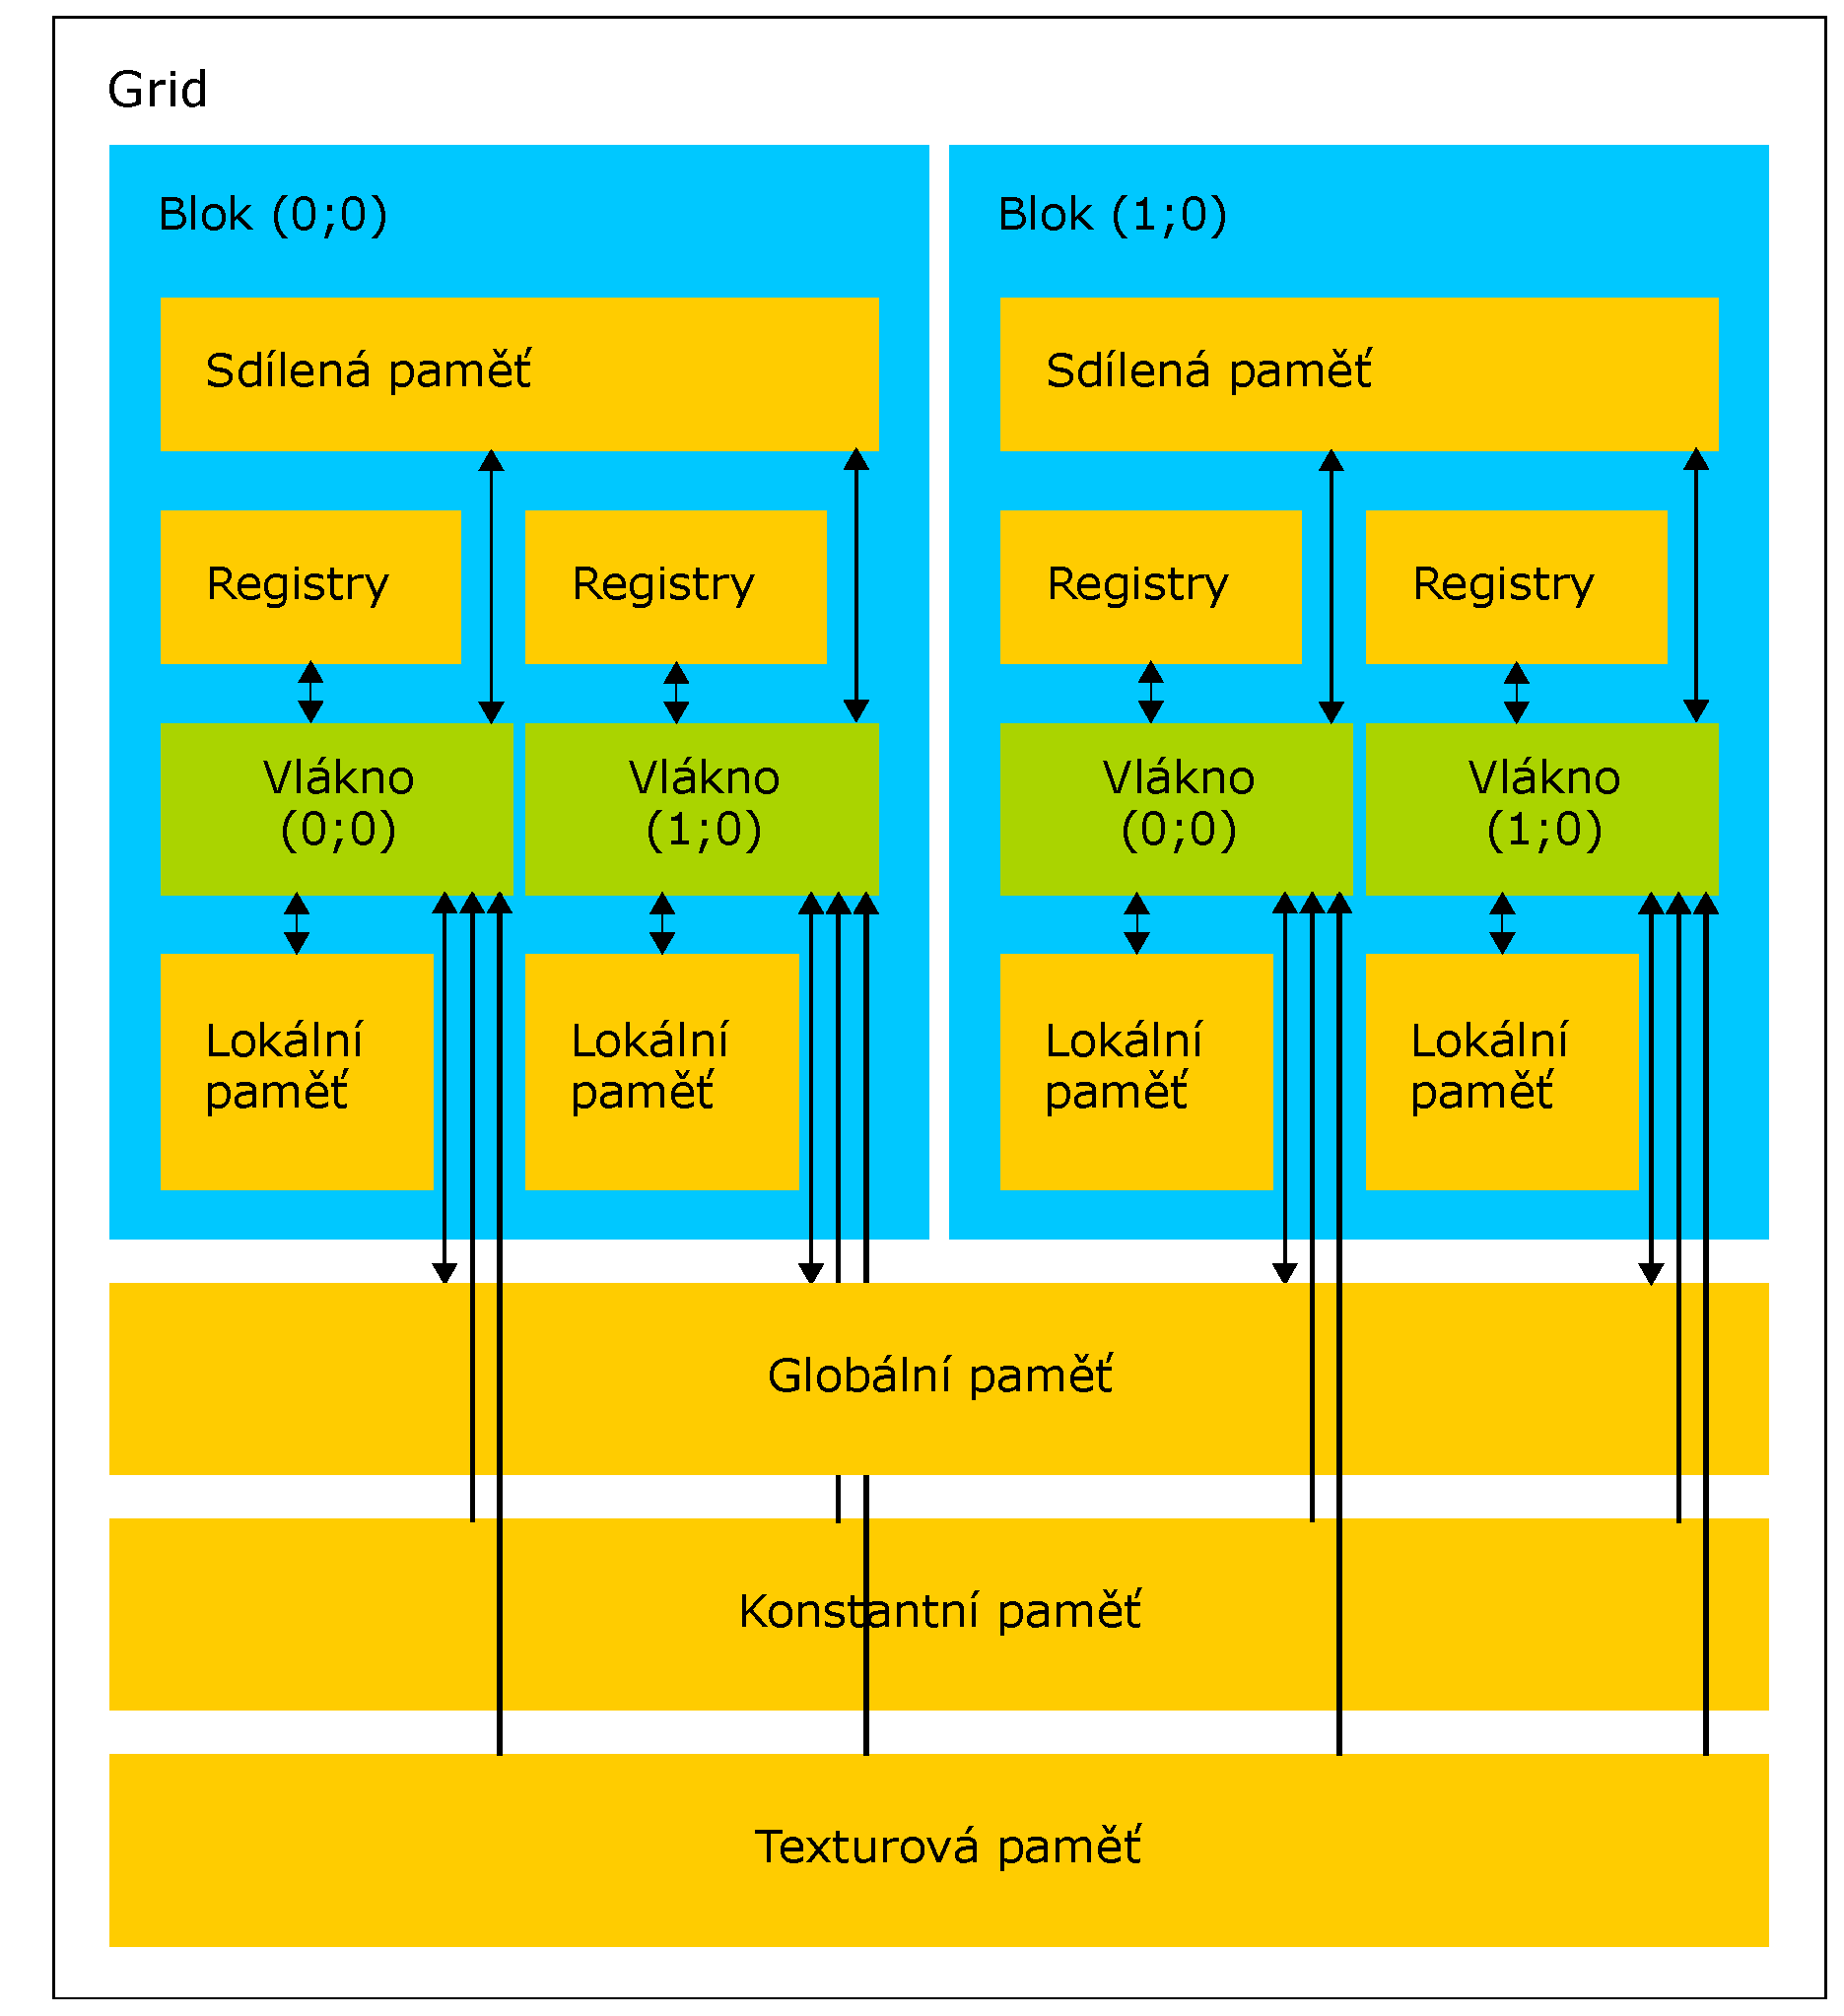
\includegraphics[width=0.6\linewidth]{img/CUDAmemAccess.eps}
  \caption{CUDA Memory access}
  \label{fig:cudamemaccess}
\end{figure}

\begin{description}
\item[Global memory] it is the largest memory (GBs) and it has high bandwidth (usually around 100 GBps) but high latency (400-600 clock cycles). It could be allocated eithe as CUDA arrays or as linear memory. CUDA arrays are opaque memory layouts optimized for texture catching. Linear memory exists on device in a 40-bit address space, so separately allocated entities ca reference another via pointers.~\cite{CUDAGuide} It is used for storing data transfered from host memory and it is allocated and released in host code by special CUDA API function before kernel launch. Global memory allocation is independent on kernel (except dynamically allocated memory inside kernel) and it could be used in many kernels without releasing and allocating new one for other kernel. Memory transfers are special host code CUDA API functions too, but they could be asynchronous. Same as memory allocation/deallocation, data are persistent between one kernel end and other kernel start. When data from this memory are accessed, they are cached in L2 cache. Also processed data or output is stored here before it is transfered back to host. It is operated in transactions of 32B - 128B so for better performance it is better to access data aligned on transaction size. Physically, it is off the chip, but on the device.

\item[Shared memory] is memory shared by all threads running on same SM. Shared memory has lower latency than global memory (32 bits / 2 cycles on CC 1.x and 2.x and 64 bits / 1 cycle on 3.x) than Global memory, but it is also smaller (depend on Compute Capability, from 16 kB on 1.x CC to 48kB on 2.x CC and 3.x CC). It could be as fast as registers if there are no bank conflicts. Shared memory has read-after write dependency which takes 24 clock cycles, but could be hidden by enough active warps. In shared memory are stored statically allocated variable or dynamic memory block could be allocated on kernel launch (it is one of kernel function parameters) and data are copied from global memory in kernel execution. Releasing of memory is done automatically after kernel is finished, so data stored here are not persistent between two kernels, they are even no persistent between same kernel re-execution.\\
This memory is divided into banks, each bank could be accessed independently which is really fast but if there are conflicts in accessing to same bank from multiple threads, access to the bank is serialized (except reading same address which is called broadcast) and could be many times slower, so for the best performance, it is better to avoid these conflicts (for example when threads accessing banks linearly~\ref{fig:linearaccess} or with stride~\ref{fig:strideaccess}, which is not a divisor of total banks count). On CC 1.x and CC 2.x, bank size is 32 bits, on CC 3.0 we can select between 32 bits and 64 bit banks. Physically it is situated near each processor for fast access.\\
\end{description}

\begin{figure}[h]
\centering
\begin{subfigure}{1.0\textwidth}
  \centering
  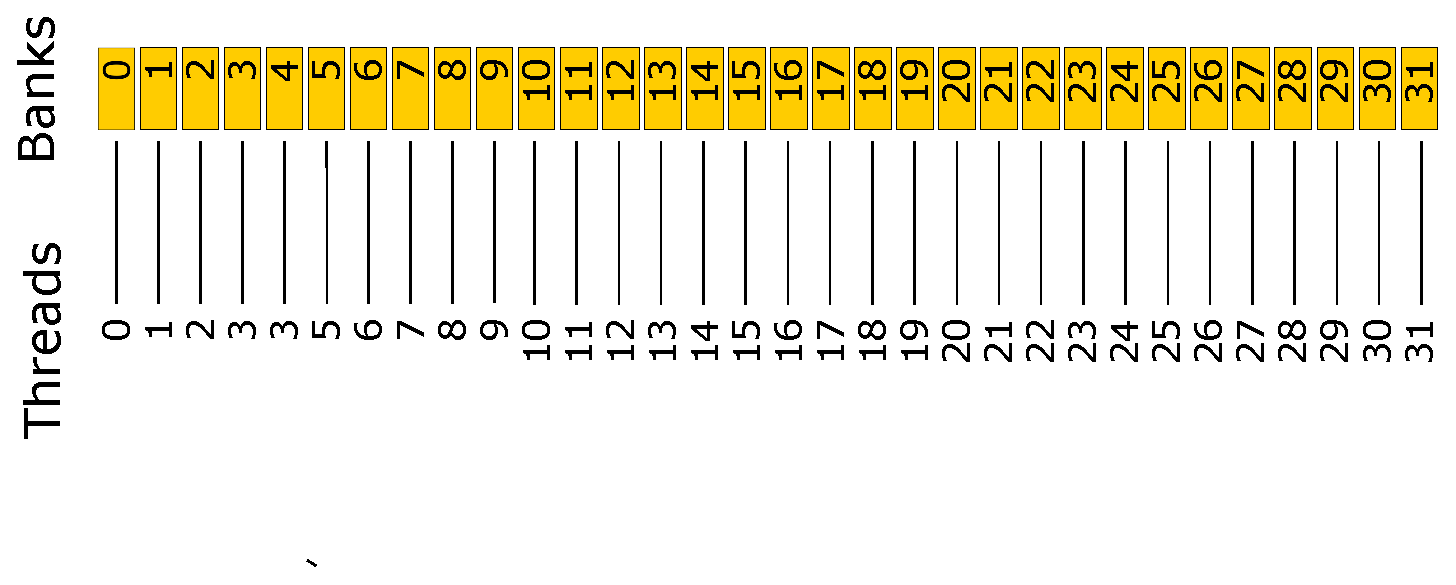
\includegraphics[width=.9\linewidth]{img/sharedMemoryLinearAccess.eps}
  \caption{Linear Access to shared memory}
  \label{fig:linearaccess}
\end{subfigure}
\begin{subfigure}{1.0\textwidth}
  \centering
  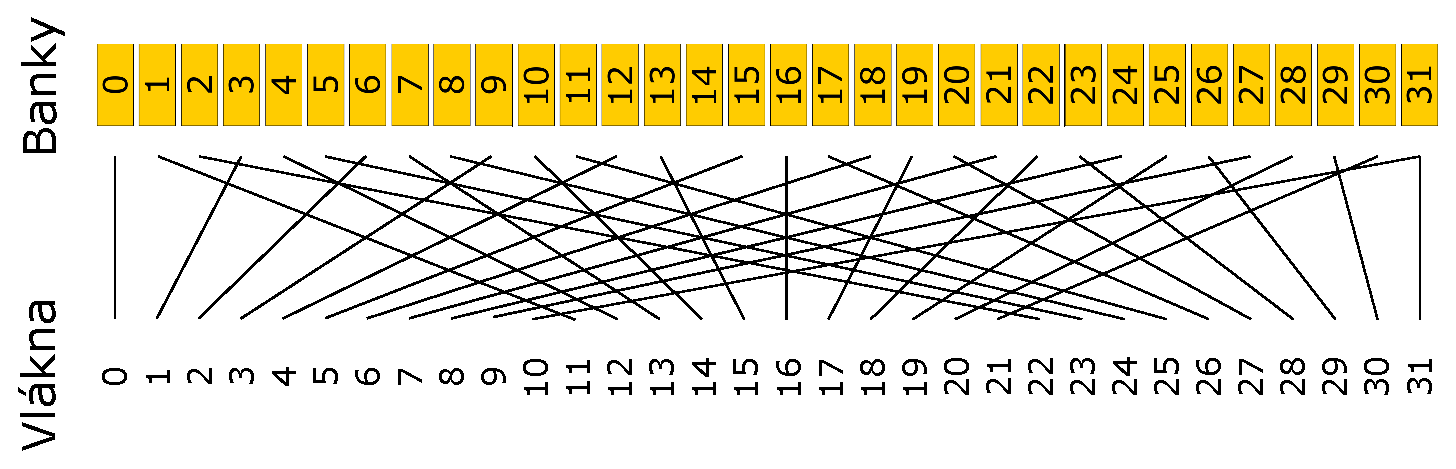
\includegraphics[width=.9\linewidth]{img/sharedMemoryStrideAccess.eps}
  \caption{Access to Shared Memory with stride 3}
  \label{fig:strideaccess}
\end{subfigure}
\caption{Shared Memory access}
\end{figure}

\begin{description}
\item[L1 Cache] has on most devices similar parameters as Share memory, because it has same resource. L1 cache is used for caching accesses to local and global memory so it could significantly speed up the memory access (100x-150x). We can configure which memory should be preferred and bigger by special CUDA API function from host code. On CC 5.0, L1 cache was merged with texture cache and is independent on shared memory (resources are not shared).
\item[Registers] Each multiprocessor has own register pool. Depend on CC, it has 8-64k of 32-bit registers. registers are the smallest memory, but also has the smallest latency (they are as fast as cores). For programmer, registers are not directly controllable. Only slow down is read-after write dependency, same as Shared memory, which takes 24 clock cycles, but it could be also hidden by enough of active warps. If kernel uses more registers than available, registers are stored to local memory. This problem is called \textit{registry spilling}.\\
Each thread has the same amount of registers. The number of registers per thread and the number of blocks determines, how many blocks could reside on SMP. For example, on CC 2.x, if kernel uses 32 registers and each block contains 512 threads, than two blocks can reside on SMP since they require $2*512*32$ registers, which exactly matches the number of registers available on SMP. If kernel uses one more register, than only single block could reside on SMP~\cite{CUDAGuide}.
\item[Local memory] is memory reserved in Global memory accessible by a single thread only. Only some automatic variables are stored in local memory~\cite{CUDAGuide}:
\begin{itemize}
\item Arrays for which it cannot determine that they are indexed with constant quantities,
\item Large structures or arrays that would consume too much register space,
\item Any variable if the kernel uses more registers than available (this is also known as register spilling).
\end{itemize}
Access to local memory are always cached by L1 and L2 memory on CC 2.x and CC 3.x. On CC 5.x, local memory accesses are always stored in L2 cache. 

\item[Constant memory] is a special memory for read-only data. Its size is 64kB and from CC 2.x, compiler stores here constant, thread-independent variables. From CC 2.x, compiler is forced to loading all constant, thread independent variables into this cache.
\item[Texture memory] is special memory used for graphics. Its benefit is 2D spatial locality used mainly for textures.
\end{description}

Data transfer between host and device are much slower than on device memory transfers (the limitation of PCI Express is 16/32 GBps depend on version, but could be slowed by host memory if the host memory is not fast enough or if source memory is swapped on disk). Memory transfer also take significant overhead, which could make CUDA inefficient for small data and compute inexpensive tasks. This problem could be solved by bulk transfers instead of individual memory transfers. Data transfer could be hidden by overlapping data transfer with computing, because CUDA device is capable of computing and simultaneously perform two asynchronous data transfers so for example, input data could be transfer for next computation step, kernel run and results from previous step could be transfered to host at one moment.\\
The host memory could be \textit{pinned} (or page locked) which could speed up memory transfer on systems with front side bus. \textit{Pinned memory} could be also used for \textit{Mapped memory} which allows eliminating memory transfers by mapping host memory into address space of device. All data transfers are than implicitly performed when data are needed by the kernel.

% is little bit different, because programmer can split execution of instructions into different branches by conditions based on thread identification. In both models
%\chapter{Implementation}
\section{Platform}
We choose a C++ language for implementing our solutions, because we need low level code optimization and features like SIMD instructions, which are not available in other languages. Even if the CUDA is developed to work with multiple languages, cooperation with  C++ is one of the best, because also CUDA kernels are written in C++. Also platform independence of C++ is useful because we developed programs on Windows and than run on Linux clusters.

\section{K-means algorithm} \label{sec:kMeansAlgorithm}
We focused on standard k-means algorithm~\cite{hartigan1979algorithm}, which input is set of $n$ points in $d$-dimensional space $R^d$ and an number of centroids $k$. The task is to assign points to centroids and minimize the distance between points and centroids. Algorithm works iteratively and each iteration consist of two steps. At first points are assigned to the nearest centroids and than new centroids are computed. Algorithm ends after known number of steps or when nothing changes between two iterations. Output of the this algorithm are centroids coordinates or points with assigned clusters.\\
As we can see in serial implementation~\autoref{lst:kMeansCode}, there are many cycles dependent on data size, so with growing number of data, serial version comes much slower. For example in two nested cycles on lines \autoref{lst:nestedCyclesBegin}-\autoref{lst:nestedCyclesEnd} of \autoref{lst:kMeansCode}, slowdown is great and this part of code is good target for parallelization.\\

\begin{lstlisting}[caption={k-means algorithm}, language=C++, escapeinside={\%*}{*)}, label={lst:kMeansCode}, numbers=left]
CreateLSH(width, hashTablesCount, basicHashFunctions)
{
  // Main iteration loop
  for( i = 0; i < iterationsCount; i++)
  {
    assign_to_clusters(data, means);
    compute_means(data_means);
  }
}

// Assign points to clusters
%*\label{lst:assignToClusters}*)assign_to_clusters(data, means)
{
//Iterate through data
%*\label{lst:nestedCyclesBegin}*)  for( d = 0; d < data_size; d++)
  {
    assigned_cluster = 0;
    min_distance = MAX_VALUE;
// Iterate through means
    for( m = 0; m < means_size; m++)
    {
      distance = count_distance( data[d], means[m] );
// If m-cluster is closer, reassign cluster
      if ( distance < min_distance )
      {
        assigned_cluster = m;
        min_distance = distance;
      }
    }
    data[d]->assigned_cluster = assigned_cluster;
%*\label{lst:nestedCyclesEnd}*)  }
}

// Compute new means
%*\label{lst:computeNewMeans}*)compute_means(data, means)
{
// Create new means array, all values are set to 0
  for( m = 0; m < means_size; m++)
  {
    new_means.push_back(new mean(0));
  }
  
// Iterate through data and accumulate data in appropriate new mean
  for( d = 0; d < data_size; d++)
  {
    assigned_cluster = data[d]->assigned_cluster;
    new_means[assigned_cluster]->contained_points++;
    for( dim = 0; dim < dimensions; dim++)
    {
      new_means[assigned_cluster]->coordinates[dim] +=
        data[d]->coordinates[dim];
    }
  }
  
// Count new means coordinates (arithmetic mean)
  for( m = 0; m < means_size; m++)
  {
    for( dim = 0; dim < dimensions; dim++)
    {
      new_means[m]->coordinates[dim] /=
        new_means[m]->contained_points;
    }
  }
}

// Function for counting distance
count_distance(point, mean)
{
  sum_squares = 0;
  for( dim = 0; dim < dimensions; dim++)
  {
    difference = point->coordinates[dim] - mean->coordinates[dim];
    sum_squares += difference * difference;
  }
  return sqrt( sum_squares );
}
\end{lstlisting}

\section{Parallelization}
As we mentioned in \autoref{sec:kMeansAlgorithm}, classical k-means algorithm contains many compute-intensive cycles, which could be parallelized. Problem is that the algorithm contains some compute dependencies, for example parallelization of nested cycles on lines \autoref{lst:nestedCyclesBegin}-\autoref{lst:nestedCyclesEnd} of \autoref{lst:kMeansCode} is problematic, because we need to accumulate coordinates in shared variable. These dependencies must be solved some way for correct parallelization.

\subsection{CPU versions}
We tried to used the most modern technologies offered by the newest CPU architectures to speed up k-means algorithm by parallelization. We created two levels of parallelization, first based on thread level (using more logical cores on single CPU) and than vectorization level using SIMD instructions.

\subsubsection{Thread level parallelization}
For thread level parallelization, we choose Threading Building Blocks (TBB) library from Intel. This library offers algorithms and data structures for parallel programing using multi-core processors but relieve programmer from complications arising from the use of native threading packages and handling particular threads. Manual thread creation, execution, synchronization and termination is hidden by using by creating TBB tasks which are processed on individual cores dynamically by the library. Also efficient use of CPU caches is automated.\\
We reworked program so points are split in groups, each group forming one TBB task.\\
\begin{description}
\item[Assigning to clusters]The first part of algorithm, assigning to clusters~\autoref{lst:kMeansCode},~\autoref{lst:assignToClusters}, is not so problematic, because only write operation is assigning cluster to point. Each point is contained in one and only one TBB task, which is processed by single thread, so it could not be read or written from other threads.\\
Second possible solution is to split means into groups and parallelize algorithm by tasks containing means. This solution is significantly slower, because we must synchronize writing information to each point about assigned cluster. If we want to remember this information in means (by accumulating assigned points to each mean) we hit a problem, because after assigning point to mean, we could not know if other mean is not closer to processed point so this way o parallelization is too computationally intensive.\\
The second part of the algorithm, counting new means~\autoref{lst:kMeansCode},~\autoref{lst:computeNewMeans}, is more problematic, because we approach means from different TBB tasks, so accumulating of coordinates must be synchronized. We solved this problem by local copy of means in each TBB task, so we avoided the collisions. For joining tasks, we used TBB reduce algorithm, when to tasks are joined, local arrays of means coordinate sums are correctly added.\\
Also in this part of algorithm exists second possible solution by approaching parallelization by splitting means. This means that for each mean, we must iterate through all points and accumulate coordinates, which means 
\end{description}
\subsubsection{Vectorization}
\subsection{GPU versions}
\section{Tools}
%\chapter{Measurements and results} \label{sec:results}

\section{Measurements}

\section{Results}


% Ukázka použití některých konstrukcí LateXu (odkomentujte, chcete-li)
% %%% Ukázka použití některých konstrukcí LaTeXud

\subsection{Ukázka \LaTeX{}u}
\label{ssec:ukazka}

This short subsection serves as an~example of basic \LaTeX{} constructs,
which can be useful for writing a~thesis.

Let us start with lists:

\begin{itemize}
\item The logo of Matfyz is displayed in figure~\ref{fig:mff}.
\item This is subsection~\ref{ssec:ukazka}.
\item Citing literature~\cite{lamport94}.
\end{itemize}

Different kinds of dashes:
red-black (short),
pages 16--22 (middle),
$45-44$ (minus),
and this is --- as you could have expected --- a~sentence-level dash,
which is the longest.
(Note that we have follwed \verb|a| by a~tilde instead of a~space
to avoid line breaks at that place.)

\newtheorem{theorem}{Theorem}
\newtheorem*{define}{Definition}	% Definice nečíslujeme, proto "*"

\begin{define}
A~{\sl Tree} is a connected graph with no cycles.
\end{define}

\begin{theorem}
This theorem is false.
\end{theorem}

\begin{proof}
False theorems do not have proofs.
\end{proof}

\begin{figure}
	\centering
	
\includegraphics[width=30mm]{../img/logo.eps}
	\caption{Logo of MFF UK}
	\label{fig:mff}
\end{figure}


\chapter*{Conclusion}
\addcontentsline{toc}{chapter}{Conclusion}


%%% Seznam použité literatury
%%% Seznam použité literatury je zpracován podle platných standardů. Povinnou citační
%%% normou pro diplomovou práci je ISO 690. Jména časopisů lze uvádět zkráceně, ale jen
%%% v kodifikované podobě. Všechny použité zdroje a prameny musí být řádně citovány.

\def\bibname{Bibliography}
\begin{thebibliography}{99}
\addcontentsline{toc}{chapter}{\bibname}

%\bibitem{lamport94}
%  {\sc Lamport,} Leslie.
%  \emph{\LaTeX: A Document Preparation System}.
%  2. vydání.
%  Massachusetts: Addison Wesley, 1994.
%  ISBN 0-201-52983-1.

\bibitem{EstivillCastro02}
{\sc Estivill-Castro,} Vladimir
\emph{Why so many clustering algorithms.}
[online]. p.~65-75. DOI 10.1145/568574.568575.

\bibitem{Zechner09}
{\sc Zechner,} Mario, {\sc Granitzer, } Michael
\emph{Accelerating K-Means on the Graphics Processor via CUDA}
First International Conference on Intensive Applications and Services
2013
ISBN: 978-1466558212 

\bibitem{Aggarwal13}
{\sc Aggarwal,} Charu C., {\sc Reddy, } Chandan K.
\emph{Data Clustering: Algorithms and Applications}
Chapman \& Hall/CRC Data Mining and Knowledge Discovery Series
2009
ISBN: 978-1-4244-3683-5

\bibitem{Drineas04}
{\sc Drineas,} P., {\sc Frieze,} A., {\sc Kannan,} R., {\sc Vempala,}  S., {\sc Vinay,}  V.
\emph{Clustering large graphs via the singular value decomposition}
Machine Learning., 56(1-3):9–33.
2004
ISSN: 0885-6125

\bibitem{Bottou95}
{\sc Bottou,} L\'{e}on, {\sc Bengio,} Yoshua
\emph{Convergence Properties of the K-Means Algorithms}
Advances in Neural Information Processing Systems 7
p.~585-592
MIT Press, 1995

\bibitem{Kim14}
{\sc Kim,} Kyoungok
\emph{Voronoi Cell-Based Clustering Using a Kernel Support.}
Knowledge and Data Engineering, IEEE Transactions
ISSN: 1041-4347
DOI 10.1109/TKDE.2014.2359662. 

\bibitem{Vallender73}
{\sc Vallender,} S.S.
\emph{Calculation of the Wasserstein Distance Between Probability Distributions on the Line.}
[online]. s.~784--786. DOI: 10.1137/1118101.

\bibitem{Beecks10}
{\sc Beecks,} Christian, {\sc Uysal,} Merih Seran, {\sc Seidl,} Thomas
\emph{Signature Quadratic Form Distance.}
Proceedings of the ACM International Conference on Image and Video Retrieval - CIVR , 2010.
ACM
ISBN 978-1-4503-0117-6
DOI 10.1145/1816041.1816105

\bibitem{Tan05}
{\sc Tan,} Pang-Ning, {\sc Michael,} Steinbach, {\sc Kumar,} Vipin
\emph{Introduction to data mining.}
Pearson New International Edition
Boston: Pearson Addison Wesley, 2005
ISBN 978-0-3213-2136-7

\bibitem{Sun15}
{\sc Sun,} Xili, {\sc Tian,} Shoucai, {\sc Lu,} Yonggang
\emph{High dimensional data clustering by partitioning the hypergraphs using dense subgraph partition}
MIPPR 2015: Pattern Recognition and Computer Vision
DOI 10.1117/12.2205743.

\bibitem{Kirk12}
{\sc Kirk,}David B., {\sc Hwu}Wen-mei W.:
\emph{Programming Massively Parallel Processors}
Second Edition: A Hands-on Approach
2012
ISBN: 0124159923 

\bibitem{Sanders10}
{\sc Sanders,} Jason, {\sc Kandrot,} Edward
\emph{CUDA by Example: An Introduction to General-Purpose GPU Programming}
NVIDIA
2010
ISBN: 0-13-138768-5 

\bibitem{Scarpino11}
{\sc Scarpino,} Matthew
\emph{OpenCL in Action: How to Accelerate Graphics and Computations}
Manning Publications
2011
ISBN: 1617290173 

\bibitem{Hong09}
{\sc Bai,} Hong-Tao, {\sc He,} Li-li, {\sc Ouyang,} Dan-tong, {\sc Li,} Zhan-shan, {\sc Li, } He
\emph{K-means on commodity GPUs with CUDA}
 Computer Science and Information Engineering
 2009
 WRI World Congress on. Volume 3.
 IEEE (2009) 651–655 

\bibitem{CUDAGuide}
Nvidia
\emph{CUDA C PROGRAMMING GUIDE}
Nvidia, 2015
available online: http://docs.nvidia.com/cuda/cuda-c-programming-guide/
\end{thebibliography}

%%% Tabulky v diplomové práci, existují-li.
\chapwithtoc{List of Tables}

%%% Použité zkratky v diplomové práci, existují-li, včetně jejich vysvětlení.
\chapwithtoc{List of Abbreviations}

%%% Přílohy k diplomové práci, existují-li (různé dodatky jako výpisy programů,
%%% diagramy apod.). Každá příloha musí být alespoň jednou odkazována z vlastního
%%% textu práce. Přílohy se číslují.
\chapwithtoc{Attachments}

\openright
\end{document}
